\documentclass[12pt]{article}

\usepackage[spanish]{babel}
\usepackage[utf8]{inputenc}
\usepackage[T1]{fontenc}
\usepackage{lmodern}
\usepackage{amsmath,amssymb}
\usepackage{siunitx}
\sisetup{output-decimal-marker={,}}
\usepackage{xcolor}
\usepackage{graphicx}
\usepackage{tikz}
\usetikzlibrary{angles,quotes,arrows.meta,calc,babel,decorations.pathmorphing}
\usepackage[a4paper,margin=2.2cm]{geometry}
\usepackage{enumitem}
\usepackage[hidelinks]{hyperref}

% ---------- Colores ----------
\definecolor{AzulFisica}{RGB}{28,74,125}
\definecolor{AzulClaro}{RGB}{235,243,251}
\definecolor{RojoFuerza}{RGB}{190,45,45}
\definecolor{VerdeRoz}{RGB}{34,120,75}
\definecolor{GrisSuave}{RGB}{245,246,248}

% ---------- Numeración automática de ejercicios ----------
\newcounter{ejercicio}
\newcommand{\ejercicio}[1]{%
  \refstepcounter{ejercicio}%
  \clearpage
  \section*{\color{AzulFisica}Ejercicio \theejercicio\ -- #1}%
  \addcontentsline{toc}{section}{Ejercicio \theejercicio: #1}%
}

\newcommand{\paso}[2]{%
  \subsection*{\color{AzulFisica}#1. #2}%
}

\setlength{\parindent}{0pt}
\setlength{\parskip}{0.45em}

\begin{document}

% ============================================================
% CARÁTULA
% ============================================================
\begin{titlepage}
\centering
\vspace*{1.8cm}

{\Large\bfseries Física Aplicada a la Tecnología de Alimentos\par}
\vspace{0.8cm}
{\color{AzulFisica}\rule{0.82\textwidth}{1.2pt}\par}
\vspace{1.3cm}

{\Huge\bfseries Unidad 3\par}
\vspace{0.25cm}
{\Huge\bfseries Dinámica\par}
\vspace{0.8cm}
{\LARGE Guía de ejercicios y ejemplos resueltos\par}

\vfill

\begin{tikzpicture}[>=Latex,scale=1.05]
  \node[font=\bfseries\large,AzulFisica] at (0,3.15) {Marco común de resolución};
  \fill[AzulClaro,rounded corners=8pt] (-5.4,-2.8) rectangle (5.4,2.45);
  \node[align=left,text width=9.2cm,font=\large] at (0,-0.1) {
  \textbf{1.} Definición del sistema en estudio\\[3pt]
  \textbf{2.} Hipótesis simplificativas\\[3pt]
  \textbf{3.} Interacciones y pares de acción--reacción\\[3pt]
  \textbf{4.} Modelo de partícula / diagrama de cuerpo libre\\[3pt]
  \textbf{5.} Planteo de la segunda ley de Newton\\[3pt]
  \textbf{6.} Resolución matemática e interpretación
  };
\end{tikzpicture}

\vfill
{\large Material de trabajo -- Unidad 3\par}
{\large 2026\par}
\end{titlepage}

\tableofcontents
\clearpage

% ============================================================
% EJERCICIO 1
% ============================================================
\ejercicio{Semáforo sostenido por tres cables}

\subsection*{Enunciado}
En la figura se muestra un semáforo que pesa \(P=\SI{125}{\newton}\) y que cuelga de un cable unido a otros dos cables fijos a un soporte. Los cables superiores forman ángulos de \(37^\circ\) y \(53^\circ\) con la horizontal. Determine la tensión en los tres cables.

\begin{center}
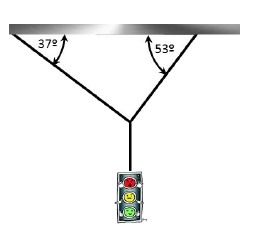
\includegraphics[width=0.48\textwidth]{semaforo.png}
\end{center}

Denominamos \(T_1\) a la tensión del cable izquierdo, \(T_2\) a la del cable derecho y \(T_3\) a la del cable vertical.

\paso{1}{Definición del sistema en estudio}
Se analizan dos sistemas:
\begin{itemize}[itemsep=2pt]
    \item \textbf{Sistema A:} el semáforo.
    \item \textbf{Sistema B:} el nudo donde se unen los tres cables.
\end{itemize}
Como el conjunto permanece en reposo, ambos sistemas están en equilibrio traslacional.

\paso{2}{Hipótesis simplificativas}
\begin{itemize}[itemsep=2pt]
    \item Tierra plana.
    \item Modelo de partícula para el semáforo y para el nudo.
    \item Cuerdas ideales: masa despreciable y tensión dirigida según el cable.
    \item Sin efecto del aire.
    \item Campo gravitatorio uniforme.
    \item Sistema en reposo: \(\vec a=\vec 0\).
\end{itemize}

\paso{3}{Interacciones y pares de acción y reacción}
Para el semáforo se identifican las interacciones Tierra--semáforo y cable vertical--semáforo. Para el nudo se identifican las interacciones entre cada uno de los tres cables y el nudo.

Los pares de acción y reacción actúan sobre cuerpos diferentes; por lo tanto, las fuerzas de un mismo par no aparecen juntas en un único diagrama de cuerpo libre.

\paso{4}{Modelos de partícula y diagramas vectoriales}

\subsubsection*{a) Modelo de partícula del semáforo}
\begin{center}
\begin{tikzpicture}[scale=1.15, >=Latex]
    \coordinate (S) at (0,0);
    \fill (S) circle (2.2pt);
    \node[right] at (0.12,0) {Semáforo};

    \draw[->,very thick,AzulFisica] (S) -- ++(90:2.2)
        node[right] {$\vec T_3$};
    \draw[->,very thick,RojoFuerza] (S) -- ++(-90:2.2)
        node[right] {$\vec P=\SI{125}{\newton}$};
\end{tikzpicture}
\end{center}

Sobre el semáforo actúan solamente \(\vec T_3\) hacia arriba y \(\vec P\) hacia abajo.

\subsubsection*{b) Modelo de partícula del nudo}
\begin{center}
\begin{tikzpicture}[scale=1.15, >=Latex]
    \coordinate (O)  at (0,0);
    \coordinate (Lh) at (-1.9,0);
    \coordinate (Lv) at ({2.8*cos(143)},{2.8*sin(143)});
    \coordinate (Rh) at (1.9,0);
    \coordinate (Rv) at ({2.8*cos(53)},{2.8*sin(53)});

    \fill (O) circle (2.2pt);
    \node[right] at (0.12,0) {Nudo};

    \draw[->,thin,gray] (-2.15,0) -- (2.15,0) node[right] {$x$};
    \draw[->,thin,gray] (0,-2.9) -- (0,2.55) node[above] {$y$};

    \draw[->,very thick,AzulFisica] (O) -- (Lv)
        node[above left] {$\vec T_1$};
    \draw[->,very thick,AzulFisica] (O) -- (Rv)
        node[above right] {$\vec T_2$};
    \draw[->,very thick,RojoFuerza] (O) -- ++(-90:2.6)
        node[right] {$\vec T_3$};

    \pic[draw, "$37^\circ$", angle radius=0.72cm, angle eccentricity=1.35]
        {angle = Lv--O--Lh};
    \pic[draw, "$53^\circ$", angle radius=0.72cm, angle eccentricity=1.35]
        {angle = Rh--O--Rv};
\end{tikzpicture}
\end{center}

\paso{5}{Planteo de la segunda ley de Newton}
Como los sistemas están en reposo,
\[
\sum \vec F = m\vec a = \vec 0.
\]

Para el semáforo:
\[
\sum F_y=0
\qquad\Rightarrow\qquad
T_3-P=0,
\]
por lo tanto,
\[
\boxed{T_3=\SI{125}{\newton}}.
\]

Para el nudo, tomando \(+x\) hacia la derecha y \(+y\) hacia arriba:
\[
\sum F_x=0
\qquad\Rightarrow\qquad
-T_1\cos 37^\circ+T_2\cos 53^\circ=0,
\]
\[
\sum F_y=0
\qquad\Rightarrow\qquad
T_1\sin 37^\circ+T_2\sin 53^\circ-T_3=0.
\]

\paso{6}{Resolución matemática e interpretación}
Como \(37^\circ+53^\circ=90^\circ\),
\[
\cos 53^\circ=\sin 37^\circ,
\qquad
\sin 53^\circ=\cos 37^\circ.
\]
Resolviendo el sistema:
\[
T_1=125\sin37^\circ\approx\SI{75.2}{\newton},
\]
\[
T_2=125\cos37^\circ\approx\SI{99.8}{\newton},
\]
\[
T_3=\SI{125}{\newton}.
\]

\[
\boxed{
T_1\approx\SI{75.2}{\newton},\qquad
T_2\approx\SI{99.8}{\newton},\qquad
T_3=\SI{125}{\newton}
}
\]

% ============================================================
% EJERCICIO 2
% ============================================================
\ejercicio{Rozamiento estático y cinético sobre una superficie horizontal}

\subsection*{Enunciado}
Un bloque que pesa \(\SI{196}{\newton}\) descansa sobre una superficie horizontal. El coeficiente estático de rozamiento entre el bloque y la superficie es \(\mu_s=0,40\), y el coeficiente cinético es \(\mu_k=0,20\).

Determinar:
\begin{enumerate}[label=\alph*)]
  \item ¿Cuál es el valor de la fuerza de rozamiento ejercida sobre el bloque?
  \item ¿Cuál será el valor de dicha fuerza si actúa sobre el bloque una fuerza horizontal de \(\SI{49}{\newton}\)?
  \item ¿Cuál es la fuerza mínima que iniciará el movimiento del bloque?
  \item ¿Cuál es la mínima fuerza que lo mantendrá en movimiento una vez iniciado este?
  \item Si la fuerza horizontal es \(\SI{98}{\newton}\), ¿cuánto valdrá la fuerza de rozamiento?
\end{enumerate}

\paso{1}{Definición del sistema en estudio}
El sistema en estudio es \textbf{el bloque}. Su peso es
\[
P=\SI{196}{\newton}.
\]
Si se desea obtener su masa,
\[
m=\frac{P}{g}=\frac{196}{9,8}=\SI{20}{\kilogram}.
\]

\paso{2}{Hipótesis simplificativas}
\begin{itemize}[itemsep=2pt]
  \item Tierra plana.
  \item El bloque se modela como una partícula para estudiar su traslación.
  \item La superficie es horizontal, rígida y no se deforma apreciablemente.
  \item Los coeficientes de rozamiento \(\mu_s\) y \(\mu_k\) se consideran constantes.
  \item Se desprecia el efecto del aire.
  \item La fuerza aplicada es horizontal.
\end{itemize}

\paso{3}{Interacciones y pares de acción y reacción}
Sobre el bloque pueden actuar las siguientes interacciones:
\begin{itemize}[itemsep=2pt]
  \item \textbf{Tierra--bloque:} la Tierra ejerce el peso \(\vec P\) sobre el bloque. El bloque ejerce sobre la Tierra una fuerza gravitatoria de igual módulo y sentido opuesto.
  \item \textbf{Superficie--bloque:} la superficie ejerce la fuerza normal \(\vec N\) y, cuando existe tendencia al deslizamiento o movimiento relativo, una fuerza de rozamiento \(\vec f\). El bloque ejerce sobre la superficie las fuerzas de reacción correspondientes.
  \item \textbf{Agente externo--bloque:} cuando se aplica una fuerza horizontal \(\vec F\), el bloque ejerce sobre el agente una fuerza de igual módulo y sentido contrario.
\end{itemize}

Un punto conceptual central es que el rozamiento estático \textbf{no vale siempre} \(\mu_sN\). Mientras no haya deslizamiento, se ajusta al valor necesario hasta un máximo:
\[
0\leq f_s\leq f_{s,\max}=\mu_sN.
\]

\paso{4}{Modelo de partícula y diagramas vectoriales}
Tomamos \(+x\) hacia la derecha y \(+y\) hacia arriba.

\subsubsection*{a) Situación estática: fuerza aplicada menor que el máximo rozamiento estático}
\begin{center}
\begin{tikzpicture}[scale=1.1,>=Latex]
  \coordinate (O) at (0,0);
  \fill (O) circle (2.3pt);
  \node[below right] at (0.08,-0.05) {bloque};

  \draw[->,thin,gray] (-3.0,0) -- (3.0,0) node[right] {$x$};
  \draw[->,thin,gray] (0,-2.5) -- (0,2.5) node[above] {$y$};

  \draw[->,very thick,AzulFisica] (O) -- ++(90:1.9) node[right] {$\vec N$};
  \draw[->,very thick,RojoFuerza] (O) -- ++(-90:1.9) node[right] {$\vec P$};
  \draw[->,very thick,AzulFisica] (O) -- ++(0:2.3) node[above] {$\vec F$};
  \draw[->,very thick,VerdeRoz] (O) -- ++(180:2.3) node[above] {$\vec f_s$};
\end{tikzpicture}
\end{center}

Mientras el bloque permanece en reposo, \(f_s\) se adapta para equilibrar a \(F\), siempre que \(F\leq f_{s,\max}\).

\subsubsection*{b) Situación cinética: bloque en deslizamiento}
\begin{center}
\begin{tikzpicture}[scale=1.1,>=Latex]
  \coordinate (O) at (0,0);
  \fill (O) circle (2.3pt);
  \node[below right] at (0.08,-0.05) {bloque};

  \draw[->,thin,gray] (-3.0,0) -- (3.3,0) node[right] {$x$};
  \draw[->,thin,gray] (0,-2.5) -- (0,2.5) node[above] {$y$};

  \draw[->,very thick,AzulFisica] (O) -- ++(90:1.9) node[right] {$\vec N$};
  \draw[->,very thick,RojoFuerza] (O) -- ++(-90:1.9) node[right] {$\vec P$};
  \draw[->,very thick,AzulFisica] (O) -- ++(0:2.8) node[above] {$\vec F$};
  \draw[->,very thick,VerdeRoz] (O) -- ++(180:1.35) node[above] {$\vec f_k$};
\end{tikzpicture}
\end{center}

Una vez iniciado el deslizamiento, el modelo emplea
\[
f_k=\mu_kN.
\]

\paso{5}{Planteo de la segunda ley de Newton}
En la dirección vertical no hay aceleración:
\[
\sum F_y=0
\qquad\Rightarrow\qquad
N-P=0.
\]
Así,
\[
\boxed{N=P=\SI{196}{\newton}}.
\]

El máximo rozamiento estático es
\[
f_{s,\max}=\mu_sN=(0,40)(196)=\SI{78.4}{\newton}.
\]

El rozamiento cinético vale
\[
f_k=\mu_kN=(0,20)(196)=\SI{39.2}{\newton}.
\]

En la dirección horizontal, la segunda ley adopta la forma general
\[
\sum F_x=ma.
\]
Mientras el bloque permanece en reposo, \(a=0\) y
\[
F-f_s=0.
\]
Durante el deslizamiento,
\[
F-f_k=ma.
\]

\paso{6}{Resolución matemática e interpretación}

\textbf{a) Bloque sin fuerza horizontal aplicada}

No existe tendencia al deslizamiento, por lo que la superficie no necesita ejercer una fuerza tangencial:
\[
\boxed{f_s=\SI{0}{\newton}}.
\]

\textbf{b) Fuerza horizontal de \(\SI{49}{\newton}\)}

Como
\[
\SI{49}{\newton}<\SI{78.4}{\newton}=f_{s,\max},
\]
el bloque permanece en reposo y el rozamiento estático se ajusta a la fuerza aplicada:
\[
\boxed{f_s=\SI{49}{\newton}}.
\]
Su sentido es opuesto a la tendencia de movimiento.

\textbf{c) Fuerza mínima que iniciará el movimiento}

El límite del equilibrio estático se alcanza cuando
\[
F=f_{s,\max}=\mu_sN.
\]
Por lo tanto, el valor umbral es
\[
\boxed{F_{\text{umbral}}=\SI{78.4}{\newton}}.
\]
Para que el movimiento efectivamente comience, la fuerza aplicada debe superar ligeramente ese valor.

\textbf{d) Fuerza mínima que lo mantendrá en movimiento una vez iniciado}

Con el bloque ya deslizándose, actúa el rozamiento cinético. Para mantener velocidad constante, \(a=0\), de modo que
\[
F=f_k=\mu_kN.
\]
Por lo tanto,
\[
\boxed{F_{\min}=\SI{39.2}{\newton}}.
\]

\textbf{e) Fuerza horizontal de \(\SI{98}{\newton}\)}

Como
\[
\SI{98}{\newton}>\SI{78.4}{\newton},
\]
se supera el máximo rozamiento estático y el bloque se desliza. En consecuencia, la fuerza de rozamiento es cinética:
\[
\boxed{f= f_k=\SI{39.2}{\newton}}.
\]

\vspace{0.5em}
\begin{center}
\fcolorbox{AzulFisica}{AzulClaro}{%
\begin{minipage}{0.88\textwidth}
\textbf{Resultados del ejercicio 2}
\[
\boxed{
\begin{aligned}
\text{a)}\;&f=\SI{0}{\newton},\\
\text{b)}\;&f=\SI{49}{\newton},\\
\text{c)}\;&F_{\text{umbral}}=\SI{78.4}{\newton},\\
\text{d)}\;&F_{\min}=\SI{39.2}{\newton},\\
\text{e)}\;&f=\SI{39.2}{\newton}.
\end{aligned}}
\]
\end{minipage}}
\end{center}


% ============================================================
% EJERCICIO 3
% ============================================================
\ejercicio{Bloque con rozamiento unido a un sistema de cuerdas}

\subsection*{Enunciado}
El bloque $A$ de la figura pesa $\SI{980}{\newton}$. El coeficiente estático de rozamiento entre el bloque y la superficie horizontal sobre la cual reposa es
\[
\mu_s=0,30.
\]
El peso colgante es $W=\SI{196}{\newton}$ y el sistema se encuentra en equilibrio.

Determinar:
\begin{enumerate}[label=\alph*)]
  \item la fuerza de rozamiento ejercida sobre el bloque $A$;
  \item el máximo peso $W$ para el cual el sistema puede permanecer en equilibrio.
\end{enumerate}

\begin{center}
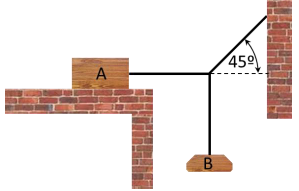
\includegraphics[width=0.62\textwidth]{ejercicio3_bloques.png}
\end{center}

\paso{1}{Definición del sistema en estudio}
Conviene separar el problema en dos sistemas:
\begin{itemize}[itemsep=2pt]
  \item \textbf{Sistema A:} el bloque $A$, apoyado sobre la superficie horizontal.
  \item \textbf{Sistema N:} el nudo ideal donde confluyen las tres cuerdas.
\end{itemize}

El peso colgante se utiliza para determinar la tensión de la cuerda vertical. Como todo el sistema está en reposo,
\[
\vec a=\vec 0.
\]

\paso{2}{Hipótesis simplificativas}
\begin{itemize}[itemsep=2pt]
  \item Tierra plana.
  \item Modelo de partícula para el bloque $A$ al estudiar su equilibrio traslacional.
  \item Nudo ideal de masa despreciable.
  \item Cuerdas ideales: masa despreciable e inextensibles.
  \item La tensión actúa en la dirección de cada cuerda.
  \item La superficie es horizontal y rígida.
  \item Se desprecia el efecto del aire.
  \item El sistema está en equilibrio estático.
\end{itemize}

\paso{3}{Interacciones y pares de acción y reacción}

\textbf{Sobre el bloque $A$:}
\begin{itemize}[itemsep=2pt]
  \item \textbf{Tierra--bloque:} la Tierra ejerce el peso $\vec P_A$ sobre el bloque; el bloque ejerce sobre la Tierra la fuerza gravitatoria de reacción.
  \item \textbf{Superficie--bloque:} la superficie ejerce la normal $\vec N$ y la fuerza de rozamiento estático $\vec f_s$; el bloque ejerce sobre la superficie las fuerzas de reacción correspondientes.
  \item \textbf{Cuerda--bloque:} la cuerda ejerce la tensión horizontal $\vec T_A$; el bloque ejerce sobre la cuerda una fuerza de igual módulo y sentido opuesto.
\end{itemize}

\textbf{Sobre el nudo:} actúan las tensiones de las tres cuerdas. Estas tres tensiones no constituyen pares de acción y reacción entre sí, porque actúan sobre el mismo sistema: el nudo.

\paso{4}{Modelo de partícula y diagramas vectoriales}
Tomamos $+x$ hacia la derecha y $+y$ hacia arriba.

\subsubsection*{a) Modelo de partícula del nudo}
\begin{center}
\begin{tikzpicture}[scale=1.15,>=Latex]
  \coordinate (O) at (0,0);
  \fill (O) circle (2.3pt);
  \node[below right] at (0.10,-0.05) {nudo};

  \draw[->,thin,gray] (-3.0,0) -- (3.0,0) node[right] {$x$};
  \draw[->,thin,gray] (0,-2.8) -- (0,2.7) node[above] {$y$};

  \draw[->,very thick,AzulFisica] (O) -- ++(180:2.45)
       node[above] {$\vec T_A$};
  \draw[->,very thick,RojoFuerza] (O) -- ++(-90:2.25)
       node[right] {$\vec T_B$};
  \draw[->,very thick,AzulFisica] (O) -- ++(45:2.85)
       node[above right] {$\vec T$};

  \coordinate (R) at (1.8,0);
  \coordinate (D) at ({2.0*cos(45)},{2.0*sin(45)});
  \pic[draw,"$45^\circ$",angle radius=0.75cm,angle eccentricity=1.35]
       {angle=R--O--D};
\end{tikzpicture}
\end{center}

Para el peso colgante, al estar en reposo,
\[
T_B=W.
\]

\subsubsection*{b) Modelo de partícula del bloque $A$}
\begin{center}
\begin{tikzpicture}[scale=1.15,>=Latex]
  \coordinate (A) at (0,0);
  \fill (A) circle (2.3pt);
  \node[below right] at (0.10,-0.05) {bloque $A$};

  \draw[->,thin,gray] (-3.0,0) -- (3.0,0) node[right] {$x$};
  \draw[->,thin,gray] (0,-2.7) -- (0,2.7) node[above] {$y$};

  \draw[->,very thick,AzulFisica] (A) -- ++(90:2.1)
       node[right] {$\vec N$};
  \draw[->,very thick,RojoFuerza] (A) -- ++(-90:2.1)
       node[right] {$\vec P_A$};
  \draw[->,very thick,AzulFisica] (A) -- ++(0:2.55)
       node[above] {$\vec T_A$};
  \draw[->,very thick,VerdeRoz] (A) -- ++(180:2.55)
       node[above] {$\vec f_s$};
\end{tikzpicture}
\end{center}

El rozamiento estático se orienta hacia la izquierda porque se opone a la tendencia del bloque a deslizarse hacia la derecha.

\paso{5}{Planteo de la segunda ley de Newton}
Como el sistema está en equilibrio,
\[
\sum\vec F=m\vec a=\vec 0.
\]

\textbf{Equilibrio del peso colgante:}
\[
\sum F_y=0
\qquad\Rightarrow\qquad
T_B-W=0,
\]
por lo tanto,
\[
\boxed{T_B=W}.
\]

\textbf{Equilibrio del nudo:}
\[
\sum F_x=0
\qquad\Rightarrow\qquad
-T_A+T\cos45^\circ=0,
\]
\[
\sum F_y=0
\qquad\Rightarrow\qquad
T\sin45^\circ-T_B=0.
\]
Como
\[
\sin45^\circ=\cos45^\circ,
\]
se obtiene
\[
\boxed{T_A=T_B=W}.
\]

\textbf{Equilibrio del bloque $A$:}

En la dirección vertical,
\[
\sum F_y=0
\qquad\Rightarrow\qquad
N-P_A=0,
\]
por lo tanto,
\[
\boxed{N=P_A=\SI{980}{\newton}}.
\]

En la dirección horizontal,
\[
\sum F_x=0
\qquad\Rightarrow\qquad
T_A-f_s=0,
\]
de modo que, mientras el bloque permanezca en equilibrio,
\[
\boxed{f_s=T_A=W}.
\]

La condición de equilibrio estático exige además
\[
f_s\leq f_{s,\max}=\mu_sN.
\]

\paso{6}{Resolución matemática e interpretación}

\textbf{a) Fuerza de rozamiento para $W=\SI{196}{\newton}$}

Del equilibrio del nudo,
\[
T_A=W=\SI{196}{\newton}.
\]
Por equilibrio horizontal del bloque,
\[
f_s=T_A.
\]
Por lo tanto,
\[
\boxed{f_s=\SI{196}{\newton}}.
\]

Verificamos que este valor sea físicamente posible. El máximo rozamiento estático disponible es
\[
f_{s,\max}=\mu_sN=(0,30)(980)=\SI{294}{\newton}.
\]
Como
\[
\SI{196}{\newton}<\SI{294}{\newton},
\]
el equilibrio es posible.

\textbf{b) Máximo peso $W$ compatible con el equilibrio}

El valor límite se alcanza cuando el rozamiento estático llega a su máximo:
\[
f_s=f_{s,\max}=\mu_sN.
\]
Como $f_s=W$,
\[
W_{\max}=\mu_sN=(0,30)(980).
\]
Así,
\[
\boxed{W_{\max}=\SI{294}{\newton}}.
\]

\vspace{0.5em}
\begin{center}
\fcolorbox{AzulFisica}{AzulClaro}{%
\begin{minipage}{0.88\textwidth}
\textbf{Resultados del ejercicio 3}
\[
\boxed{
\begin{aligned}
\text{a)}\;&f_s=\SI{196}{\newton},\\
\text{b)}\;&W_{\max}=\SI{294}{\newton}.
\end{aligned}}
\]
\end{minipage}}
\end{center}

\textbf{Interpretación física.} Para $W=\SI{196}{\newton}$, el rozamiento estático necesario es menor que el máximo disponible. Al aumentar $W$, aumenta en igual proporción la tensión horizontal sobre el bloque. Cuando $W$ alcanza $\SI{294}{\newton}$, el rozamiento estático está en su valor límite; un incremento adicional del peso provoca el inicio del deslizamiento del bloque $A$.



% ============================================================
% EJERCICIO 4
% ============================================================
\ejercicio{Bloques con rozamiento cinético en tres configuraciones}

\subsection*{Enunciado}
El bloque $A$ de la figura pesa $\SI{39.2}{\newton}$ y el bloque $B$, $\SI{78.4}{\newton}$. El coeficiente cinético de rozamiento entre todas las superficies es
\[
\mu_k=0,25.
\]
Calcular la fuerza $F$ necesaria para arrastrar el bloque $B$ hacia la izquierda con velocidad constante:
\begin{enumerate}[label=\alph*)]
  \item si $A$ descansa sobre $B$ y se mueve con él;
  \item si $A$ se mantiene en reposo;
  \item si $A$ y $B$ están unidos por una cuerda ligera y flexible que pasa por una polea fija sin rozamiento.
\end{enumerate}

\begin{center}
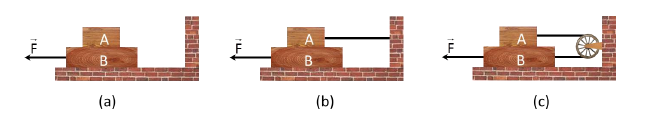
\includegraphics[width=0.92\textwidth]{ejercicio4_arrastre.png}
\end{center}

\paso{1}{Definición del sistema en estudio}
Como el ejercicio presenta tres configuraciones, conviene trabajar en cada inciso con los sistemas estrictamente necesarios:
\begin{itemize}[itemsep=2pt]
  \item en el inciso \textbf{a)}, el sistema puede considerarse como el conjunto $A+B$;
  \item en el inciso \textbf{b)}, se analiza principalmente el bloque $B$, teniendo en cuenta además la interacción de rozamiento con $A$;
  \item en el inciso \textbf{c)}, se analizan por separado los bloques $A$ y $B$, ya que además de las fuerzas de rozamiento interviene la tensión de la cuerda.
\end{itemize}

En los tres casos, el bloque $B$ se desplaza hacia la izquierda con velocidad constante. Por lo tanto,
\[
\vec a=\vec 0.
\]

\paso{2}{Hipótesis simplificativas}
\begin{itemize}[itemsep=2pt]
  \item Tierra plana.
  \item Modelo de partícula para ambos bloques.
  \item Superficies rígidas.
  \item Rozamiento cinético con coeficiente constante $\mu_k=0,25$ entre todas las superficies en contacto donde existe deslizamiento relativo.
  \item Cuerda ideal y polea ideal en el inciso \textbf{c)}.
  \item Se desprecia el efecto del aire.
  \item El movimiento se produce con velocidad constante, de modo que la resultante horizontal es nula.
\end{itemize}

Los pesos de los bloques son:
\[
P_A=\SI{39.2}{\newton},
\qquad
P_B=\SI{78.4}{\newton}.
\]
Las masas resultan:
\[
m_A=\frac{39.2}{9.8}=\SI{4}{\kilogram},
\qquad
m_B=\frac{78.4}{9.8}=\SI{8}{\kilogram}.
\]

\paso{3}{Interacciones y pares de acción y reacción}
Las interacciones relevantes son:
\begin{itemize}[itemsep=2pt]
  \item \textbf{Tierra--bloques:} originan los pesos $\vec P_A$ y $\vec P_B$.
  \item \textbf{Bloque $B$--suelo:} originan la normal del suelo sobre $B$ y el rozamiento cinético suelo--$B$.
  \item \textbf{Bloque $A$--bloque $B$:} originan la normal mutua y, cuando hay deslizamiento relativo, el rozamiento cinético entre ambos bloques.
  \item \textbf{Cuerda--bloques:} en el inciso \textbf{c)}, la cuerda ejerce una tensión $\vec T$ sobre cada bloque.
  \item \textbf{Agente externo--bloque $B$:} origina la fuerza aplicada $\vec F$ hacia la izquierda.
\end{itemize}

Recordemos que los pares de acción y reacción actúan sobre cuerpos distintos; por eso, en el diagrama de cuerpo libre de cada bloque sólo aparecen las fuerzas \emph{que actúan sobre ese bloque}.

\paso{4}{Modelo de partícula y diagramas vectoriales}
Primero se calcula la fuerza de rozamiento del bloque $B$ con el piso. Como el bloque $A$ está apoyado sobre $B$, la normal del piso vale
\[
N_{\text{piso}}=P_A+P_B=39.2+78.4=\SI{117.6}{\newton}.
\]
Por lo tanto, el rozamiento cinético del piso sobre $B$ es
\[
f_{k,\text{piso}}=\mu_kN_{\text{piso}}=(0.25)(117.6)=\SI{29.4}{\newton}.
\]

Además, cuando existe deslizamiento relativo entre $A$ y $B$, la normal entre ellos es
\[
N_{AB}=P_A=\SI{39.2}{\newton},
\]
y entonces el rozamiento cinético entre ambos bloques tiene módulo
\[
f_{k,AB}=\mu_kN_{AB}=(0.25)(39.2)=\SI{9.8}{\newton}.
\]

\subsubsection*{a) $A$ se mueve junto con $B$}
Si ambos bloques se desplazan juntos, no hay movimiento relativo entre $A$ y $B$. En consecuencia, para este inciso no interviene rozamiento cinético entre ellos. El sistema relevante es el conjunto $A+B$:

\begin{center}
\begin{tikzpicture}[scale=1.1,>=Latex]
  \coordinate (O) at (0,0);
  \fill (O) circle (2.3pt);
  \node[below right] at (0.08,-0.05) {$A+B$};

  \draw[->,thin,gray] (-3.1,0) -- (3.1,0) node[right] {$x$};
  \draw[->,thin,gray] (0,-2.5) -- (0,2.5) node[above] {$y$};

  \draw[->,very thick,AzulFisica] (O) -- ++(180:2.5) node[above] {$\vec F$};
  \draw[->,very thick,VerdeRoz] (O) -- ++(0:2.5) node[above] {$\vec f_{k,\text{piso}}$};
  \draw[->,very thick,AzulFisica] (O) -- ++(90:1.9) node[right] {$\vec N$};
  \draw[->,very thick,RojoFuerza] (O) -- ++(-90:1.9) node[right] {$\vec P_A+\vec P_B$};
\end{tikzpicture}
\end{center}

\subsubsection*{b) $A$ se mantiene en reposo}
En este caso el bloque $B$ se desliza hacia la izquierda bajo el bloque $A$. El diagrama relevante para $B$ es:

\begin{center}
\begin{tikzpicture}[scale=1.1,>=Latex]
  \coordinate (O) at (0,0);
  \fill (O) circle (2.3pt);
  \node[below right] at (0.08,-0.05) {$B$};

  \draw[->,thin,gray] (-3.3,0) -- (3.3,0) node[right] {$x$};
  \draw[->,thin,gray] (0,-2.6) -- (0,2.6) node[above] {$y$};

  \draw[->,very thick,AzulFisica] (O) -- ++(180:2.8) node[above] {$\vec F$};
  \draw[->,very thick,VerdeRoz] (O) -- ++(0:2.0) node[above] {$\vec f_{k,AB}$};
  \draw[->,very thick,VerdeRoz] (O) -- ++(0:2.9) node[below=2pt] {$\vec f_{k,\text{piso}}$};
  \draw[->,very thick,AzulFisica] (O) -- ++(90:2.0) node[right] {$\vec N_{\text{piso}}$};
  \draw[->,very thick,RojoFuerza] (O) -- ++(-90:2.0) node[right] {$\vec P_A+\vec P_B$};
\end{tikzpicture}
\end{center}

Como $B$ se mueve hacia la izquierda respecto de $A$, el rozamiento que $A$ ejerce sobre $B$ apunta hacia la derecha.

\subsubsection*{c) $A$ y $B$ unidos por una cuerda y polea}
En esta configuración, si $B$ se desplaza hacia la izquierda con rapidez constante, la cuerda obliga a que $A$ se desplace hacia la derecha con igual rapidez. Por ello existe deslizamiento relativo entre ambos bloques.

\begin{center}
\begin{tikzpicture}[scale=1.05,>=Latex]
  % Bloque A
  \coordinate (A) at (-3.4,0);
  \fill (A) circle (2.2pt);
  \node[below left] at (-3.32,-0.05) {$A$};
  \draw[->,very thick,AzulFisica] (A) -- ++(0:2.3) node[above] {$\vec T$};
  \draw[->,very thick,VerdeRoz] (A) -- ++(180:2.0) node[above] {$\vec f_{k,AB}$};
  \draw[->,very thick,AzulFisica] (A) -- ++(90:1.6) node[right] {$\vec N_{AB}$};
  \draw[->,very thick,RojoFuerza] (A) -- ++(-90:1.6) node[right] {$\vec P_A$};

  % Bloque B
  \coordinate (B) at (3.0,0);
  \fill (B) circle (2.2pt);
  \node[below right] at (3.08,-0.05) {$B$};
  \draw[->,very thick,AzulFisica] (B) -- ++(180:2.5) node[above] {$\vec F$};
  \draw[->,very thick,AzulFisica] (B) -- ++(0:1.8) node[above] {$\vec T$};
  \draw[->,very thick,VerdeRoz] (B) -- ++(0:2.4) node[above] {$\vec f_{k,\text{piso}}$};
  \draw[->,very thick,VerdeRoz] (B) -- ++(0:1.2) node[below=2pt] {$\vec f_{k,AB}$};
  \draw[->,very thick,AzulFisica] (B) -- ++(90:1.8) node[right] {$\vec N_{\text{piso}}$};
  \draw[->,very thick,RojoFuerza] (B) -- ++(-90:1.8) node[right] {$\vec P_A+\vec P_B$};
\end{tikzpicture}
\end{center}

\paso{5}{Planteo de la segunda ley de Newton}
En todos los casos el movimiento es con velocidad constante, por lo tanto
\[
\sum \vec F = m\vec a = \vec 0.
\]

\textbf{Inciso a)} Considerando el sistema $A+B$ y proyectando sobre el eje horizontal:
\[
-F+f_{k,\text{piso}}=0
\qquad\Rightarrow\qquad
F=f_{k,\text{piso}}.
\]

\textbf{Inciso b)} Para el bloque $B$:
\[
-F+f_{k,\text{piso}}+f_{k,AB}=0,
\]
de donde
\[
F=f_{k,\text{piso}}+f_{k,AB}.
\]

\textbf{Inciso c)}

Para el bloque $A$:
\[
\sum F_x=0
\qquad\Rightarrow\qquad
T-f_{k,AB}=0,
\]
por lo tanto,
\[
T=f_{k,AB}.
\]

Para el bloque $B$:
\[
-F+f_{k,\text{piso}}+f_{k,AB}+T=0,
\]
por lo tanto,
\[
F=f_{k,\text{piso}}+f_{k,AB}+T.
\]

\paso{6}{Resolución matemática e interpretación}

\textbf{a) Si $A$ descansa sobre $B$ y se mueve con él}
\[
F=f_{k,\text{piso}}=\SI{29.4}{\newton}.
\]
Así,
\[
\boxed{F=\SI{29.4}{\newton}}.
\]

\textbf{Interpretación.} Como no hay deslizamiento relativo entre $A$ y $B$, no aparece rozamiento cinético entre ellos; la única resistencia horizontal externa al sistema es la del piso.

\textbf{b) Si $A$ se mantiene en reposo}
\[
F=f_{k,\text{piso}}+f_{k,AB}=29.4+9.8=\SI{39.2}{\newton}.
\]
Por lo tanto,
\[
\boxed{F=\SI{39.2}{\newton}}.
\]

\textbf{Interpretación.} Ahora el bloque $B$ no sólo debe vencer el rozamiento con el piso, sino también el rozamiento cinético con el bloque superior $A$, que se opone al deslizamiento relativo.

\textbf{c) Si $A$ y $B$ están unidos por una cuerda y polea}
Primero, del equilibrio horizontal del bloque $A$:
\[
T=f_{k,AB}=\SI{9.8}{\newton}.
\]
Entonces,
\[
F=f_{k,\text{piso}}+f_{k,AB}+T=29.4+9.8+9.8=\SI{49.0}{\newton}.
\]
De modo que
\[
\boxed{F=\SI{49.0}{\newton}}.
\]

\textbf{Interpretación.} En esta configuración, además del rozamiento con el piso y del rozamiento entre bloques, la fuerza aplicada debe compensar la tensión de la cuerda. Esa tensión tiene el mismo módulo que el rozamiento que actúa sobre el bloque $A$.

\vspace{0.5em}
\begin{center}
\fcolorbox{AzulFisica}{AzulClaro}{%
\begin{minipage}{0.88\textwidth}
\textbf{Resultados del ejercicio 4}
\[
\boxed{
\begin{aligned}
\text{a)}\;&F=\SI{29.4}{\newton},\\
\text{b)}\;&F=\SI{39.2}{\newton},\\
\text{c)}\;&F=\SI{49.0}{\newton}.
\end{aligned}}
\]
\end{minipage}}
\end{center}


% ============================================================
% EJERCICIO 5
% ============================================================
\ejercicio{Lectura de una balanza de resorte dentro de un ascensor}

\subsection*{Enunciado}
Un cuerpo pende de una balanza de resorte sujeta al techo de un ascensor.

Determinar:
\begin{enumerate}[label=\alph*)]
  \item si el ascensor tiene una aceleración hacia arriba de $\SI{1.20}{\meter\per\second\squared}$ y la balanza indica $\SI{220}{\newton}$, ¿cuál es el verdadero peso del cuerpo?;
  \item ¿en qué circunstancias indicará la balanza $\SI{175}{\newton}$?;
  \item ¿qué indicará la balanza si se rompe el cable del ascensor?
\end{enumerate}

\paso{1}{Definición del sistema en estudio}
El sistema en estudio es \textbf{el cuerpo suspendido de la balanza}. La lectura de la balanza corresponde al módulo de la tensión $T$ que el resorte ejerce sobre el cuerpo.

Tomamos como eje $y$ la dirección vertical y elegimos el sentido positivo hacia arriba.

\paso{2}{Hipótesis simplificativas}
\begin{itemize}[itemsep=2pt]
  \item Tierra plana.
  \item Modelo de partícula para el cuerpo.
  \item Balanza ideal: su lectura es igual a la tensión $T$ del resorte.
  \item Se desprecia el efecto del aire.
  \item Campo gravitatorio uniforme, con $g=\SI{9.8}{\meter\per\second\squared}$.
  \item El ascensor y el cuerpo poseen la misma aceleración mientras el cuerpo permanece suspendido de la balanza.
\end{itemize}

\paso{3}{Interacciones y pares de acción y reacción}
Sobre el cuerpo actúan dos interacciones:
\begin{itemize}[itemsep=2pt]
  \item \textbf{Tierra--cuerpo:} la Tierra ejerce el peso $\vec P=m\vec g$ hacia abajo; el cuerpo ejerce sobre la Tierra la correspondiente fuerza gravitatoria de reacción.
  \item \textbf{Balanza--cuerpo:} la balanza ejerce la tensión $\vec T$ hacia arriba; el cuerpo ejerce sobre la balanza una fuerza de igual módulo y sentido opuesto.
\end{itemize}

La lectura de la balanza no es, en general, igual al peso del cuerpo: representa la \textbf{fuerza de contacto} que la balanza ejerce sobre él.

\paso{4}{Modelo de partícula y diagramas vectoriales}

\subsubsection*{a) Ascensor con aceleración hacia arriba}
\begin{center}
\begin{tikzpicture}[scale=1.05,>=Latex]
  \coordinate (O) at (0,0);
  \fill (O) circle (2.3pt);
  \node[below right] at (0.08,-0.05) {cuerpo};
  \draw[->,thin,gray] (0,-2.5) -- (0,2.8) node[above] {$y$};
  \draw[->,very thick,AzulFisica] (O) -- ++(90:2.15) node[right] {$\vec T$};
  \draw[->,very thick,RojoFuerza] (O) -- ++(-90:1.75) node[right] {$\vec P$};
  \draw[->,thick,dashed] (1.45,0) -- ++(90:1.35) node[right] {$\vec a$};
\end{tikzpicture}
\end{center}

\subsubsection*{b) Lectura menor que el peso verdadero}
\begin{center}
\begin{tikzpicture}[scale=1.05,>=Latex]
  \coordinate (O) at (0,0);
  \fill (O) circle (2.3pt);
  \node[below right] at (0.08,-0.05) {cuerpo};
  \draw[->,thin,gray] (0,-2.8) -- (0,2.5) node[above] {$y$};
  \draw[->,very thick,AzulFisica] (O) -- ++(90:1.55) node[right] {$\vec T$};
  \draw[->,very thick,RojoFuerza] (O) -- ++(-90:2.05) node[right] {$\vec P$};
  \draw[->,thick,dashed] (1.45,0) -- ++(-90:1.35) node[right] {$\vec a$};
\end{tikzpicture}
\end{center}

\subsubsection*{c) Cable del ascensor roto: caída libre}
Mientras el ascensor, la balanza y el cuerpo caen libremente, todos poseen la aceleración gravitatoria. La balanza deja de estar cargada y su lectura se hace nula.

\begin{center}
\begin{tikzpicture}[scale=1.05,>=Latex]
  \coordinate (O) at (0,0);
  \fill (O) circle (2.3pt);
  \node[below right] at (0.08,-0.05) {cuerpo};
  \draw[->,thin,gray] (0,-2.8) -- (0,2.0) node[above] {$y$};
  \draw[->,very thick,RojoFuerza] (O) -- ++(-90:2.05) node[right] {$\vec P$};
  \draw[->,thick,dashed] (1.45,0) -- ++(-90:1.75) node[right] {$\vec a=\vec g$};
  \node[AzulFisica] at (-1.7,1.35) {$T=0$};
\end{tikzpicture}
\end{center}

\paso{5}{Planteo de la segunda ley de Newton}
Con $+y$ hacia arriba,
\[
\sum F_y=ma_y.
\]
Por lo tanto,
\[
T-P=ma_y,
\]
y como $P=mg$,
\[
\boxed{T=m(g+a_y)}.
\]
Esta expresión permite interpretar directamente la lectura de la balanza:
\begin{itemize}[itemsep=2pt]
  \item si $a_y>0$, entonces $T>P$;
  \item si $a_y=0$, entonces $T=P$;
  \item si $a_y<0$, entonces $T<P$;
  \item si $a_y=-g$, entonces $T=0$.
\end{itemize}

\paso{6}{Resolución matemática e interpretación}

\textbf{a) Verdadero peso del cuerpo}

La balanza indica
\[
T=\SI{220}{\newton}
\]
y la aceleración es hacia arriba:
\[
a_y=+\SI{1.20}{\meter\per\second\squared}.
\]
Entonces,
\[
220=m(9.8+1.20)=11.0m,
\]
de donde
\[
m=\SI{20.0}{\kilogram}.
\]
El peso verdadero es
\[
P=mg=(20.0)(9.8)=\SI{196}{\newton}.
\]
Por lo tanto,
\[
\boxed{P=\SI{196}{\newton}}.
\]

\textbf{b) Circunstancias para que la balanza indique $\SI{175}{\newton}$}

Con $m=\SI{20.0}{\kilogram}$,
\[
175=20.0(9.8+a_y).
\]
Por lo tanto,
\[
8.75=9.8+a_y,
\]
\[
a_y=-\SI{1.05}{\meter\per\second\squared}.
\]
Así,
\[
\boxed{a=\SI{1.05}{\meter\per\second\squared}\ \text{hacia abajo}}.
\]

La balanza indicará $\SI{175}{\newton}$ siempre que el ascensor tenga esa aceleración hacia abajo. Esto puede ocurrir, por ejemplo, cuando el ascensor \textbf{desciende aumentando su rapidez} o cuando \textbf{asciende disminuyendo su rapidez}.

\textbf{c) Lectura si se rompe el cable del ascensor}

En caída libre,
\[
a_y=-g.
\]
Entonces,
\[
T=m(g-g)=0.
\]
Por lo tanto,
\[
\boxed{T=\SI{0}{\newton}}.
\]

\textbf{Interpretación.} El cuerpo no pierde su peso gravitatorio: la Tierra sigue ejerciendo $P=mg$. Lo que desaparece es la tensión de la balanza. Ésta es la condición de \textbf{ingravidez aparente}.

\vspace{0.5em}
\begin{center}
\fcolorbox{AzulFisica}{AzulClaro}{%
\begin{minipage}{0.88\textwidth}
\textbf{Resultados del ejercicio 5}
\[
\boxed{
\begin{aligned}
\text{a)}\;&P=\SI{196}{\newton},\\
\text{b)}\;&a=\SI{1.05}{\meter\per\second\squared}\ \text{hacia abajo},\\
\text{c)}\;&T=\SI{0}{\newton}.
\end{aligned}}
\]
\end{minipage}}
\end{center}

% ============================================================
% EJERCICIO 6
% ============================================================
\ejercicio{Caja sobre la plataforma de un camión acelerado}

\subsection*{Enunciado}
Una caja de embalaje de $\SI{40}{\kilogram}$ se encuentra sobre el piso de la plataforma de un camión. El coeficiente estático de rozamiento entre la caja y la plataforma es
\[
\mu_s=0,30,
\]
y el coeficiente cinético es
\[
\mu_k=0,20.
\]

Calcular la magnitud y el sentido de la fuerza de rozamiento que actúa sobre la caja:
\begin{enumerate}[label=\alph*)]
  \item cuando el camión tiene una aceleración de $\SI{1.80}{\meter\per\second\squared}$;
  \item cuando su desaceleración es de $\SI{3.00}{\meter\per\second\squared}$.
\end{enumerate}

\paso{1}{Definición del sistema en estudio}
El sistema en estudio es \textbf{la caja}. Para que permanezca sin deslizar respecto de la plataforma, debe adquirir la misma aceleración horizontal que el camión. La fuerza horizontal que puede producir esa aceleración es la fuerza de rozamiento ejercida por la plataforma sobre la caja.

\paso{2}{Hipótesis simplificativas}
\begin{itemize}[itemsep=2pt]
  \item Tierra plana.
  \item Modelo de partícula para la caja.
  \item Plataforma horizontal y rígida.
  \item Coeficientes de rozamiento constantes.
  \item Se desprecia el efecto del aire.
  \item Mientras no haya deslizamiento, actúa rozamiento estático; si la caja desliza respecto de la plataforma, actúa rozamiento cinético.
\end{itemize}

\paso{3}{Interacciones y pares de acción y reacción}
Sobre la caja actúan:
\begin{itemize}[itemsep=2pt]
  \item \textbf{Tierra--caja:} peso $\vec P=m\vec g$ hacia abajo.
  \item \textbf{Plataforma--caja:} normal $\vec N$ hacia arriba y fuerza de rozamiento horizontal $\vec f$.
\end{itemize}

El rozamiento es la interacción que modifica el movimiento horizontal de la caja. Su sentido se determina por la \textbf{tendencia al deslizamiento relativo}, no simplemente por el sentido de la velocidad del camión.

\paso{4}{Modelo de partícula y diagramas vectoriales}
En la dirección vertical no hay aceleración, de modo que
\[
N=mg=(40)(9.8)=\SI{392}{\newton}.
\]

Por lo tanto,
\[
f_{s,\max}=\mu_sN=(0.30)(392)=\SI{117.6}{\newton},
\]
y, si se produce deslizamiento,
\[
f_k=\mu_kN=(0.20)(392)=\SI{78.4}{\newton}.
\]

\subsubsection*{a) Camión acelerando}
El rozamiento sobre la caja debe apuntar en el mismo sentido que la aceleración del camión para acelerar la caja junto con la plataforma.

\begin{center}
\begin{tikzpicture}[scale=1.05,>=Latex]
  \coordinate (O) at (0,0);
  \fill (O) circle (2.3pt);
  \node[below right] at (0.08,-0.05) {caja};
  \draw[->,thin,gray] (-2.8,0) -- (3.2,0) node[right] {$x$};
  \draw[->,thin,gray] (0,-2.5) -- (0,2.5) node[above] {$y$};
  \draw[->,very thick,VerdeRoz] (O) -- ++(0:2.35) node[above] {$\vec f_s$};
  \draw[->,very thick,AzulFisica] (O) -- ++(90:1.8) node[right] {$\vec N$};
  \draw[->,very thick,RojoFuerza] (O) -- ++(-90:1.8) node[right] {$\vec P$};
  \draw[->,thick,dashed] (0.1,-1.2) -- ++(0:1.55) node[below] {$\vec a$};
\end{tikzpicture}
\end{center}

\subsubsection*{b) Camión desacelerando}
Supongamos que el camión se desplaza hacia adelante y está frenando. Su aceleración apunta hacia atrás. La caja tiende a continuar moviéndose hacia adelante respecto de la plataforma; por eso el rozamiento sobre la caja apunta \textbf{hacia atrás}, es decir, en el sentido de la desaceleración del camión.

\begin{center}
\begin{tikzpicture}[scale=1.05,>=Latex]
  \coordinate (O) at (0,0);
  \fill (O) circle (2.3pt);
  \node[below right] at (0.08,-0.05) {caja};
  \draw[->,thin,gray] (-3.2,0) -- (2.8,0) node[right] {$x$};
  \draw[->,thin,gray] (0,-2.5) -- (0,2.5) node[above] {$y$};
  \draw[->,very thick,VerdeRoz] (O) -- ++(180:2.2) node[above] {$\vec f_k$};
  \draw[->,very thick,AzulFisica] (O) -- ++(90:1.8) node[right] {$\vec N$};
  \draw[->,very thick,RojoFuerza] (O) -- ++(-90:1.8) node[right] {$\vec P$};
  \draw[->,thick,dashed] (-0.1,-1.2) -- ++(180:1.55) node[below] {$\vec a_{\text{camión}}$};
\end{tikzpicture}
\end{center}

\paso{5}{Planteo de la segunda ley de Newton}
Horizontalmente,
\[
\sum F_x=ma_x.
\]
Si la caja no desliza respecto del camión, la fuerza necesaria es
\[
f_s=ma.
\]
Pero esta condición sólo puede cumplirse si
\[
f_s\leq f_{s,\max}.
\]
Si la fuerza necesaria supera el máximo rozamiento estático, la caja desliza y entonces la fuerza de rozamiento pasa a ser
\[
f_k=\mu_kN.
\]

\paso{6}{Resolución matemática e interpretación}

\textbf{a) Aceleración del camión de $\SI{1.80}{\meter\per\second\squared}$}

La fuerza necesaria para que la caja acompañe al camión es
\[
f_{\text{necesaria}}=ma=(40)(1.80)=\SI{72.0}{\newton}.
\]
Como
\[
\SI{72.0}{\newton}<\SI{117.6}{\newton}=f_{s,\max},
\]
no hay deslizamiento. La fuerza de rozamiento es estática y vale
\[
\boxed{f_s=\SI{72.0}{\newton}}.
\]
Su sentido es \textbf{el mismo que el de la aceleración del camión}.

\textbf{b) Desaceleración del camión de $\SI{3.00}{\meter\per\second\squared}$}

Para que la caja acompañara al camión sin deslizar sería necesaria una fuerza de módulo
\[
f_{\text{necesaria}}=ma=(40)(3.00)=\SI{120}{\newton}.
\]
Pero
\[
\SI{120}{\newton}>\SI{117.6}{\newton}=f_{s,\max}.
\]
El rozamiento estático no alcanza para impedir el deslizamiento. Por lo tanto, la caja desliza respecto de la plataforma y actúa rozamiento cinético:
\[
f_k=\mu_kN=(0.20)(392)=\SI{78.4}{\newton}.
\]
Así,
\[
\boxed{f_k=\SI{78.4}{\newton}}.
\]
Su sentido es \textbf{hacia atrás}, es decir, en el sentido de la desaceleración del camión y opuesto a la tendencia de la caja a deslizar hacia adelante respecto de la plataforma.

Como comprobación, la aceleración real de la caja mientras desliza es
\[
a_{\text{caja}}=\frac{f_k}{m}=\frac{78.4}{40}=\SI{1.96}{\meter\per\second\squared},
\]
menor que la desaceleración del camión, lo que explica que la caja avance respecto de la plataforma durante el frenado.

\vspace{0.5em}
\begin{center}
\fcolorbox{AzulFisica}{AzulClaro}{%
\begin{minipage}{0.88\textwidth}
\textbf{Resultados del ejercicio 6}
\[
\boxed{
\begin{aligned}
\text{a)}\;&f_s=\SI{72.0}{\newton},\quad \text{en el sentido de la aceleración},\\
\text{b)}\;&f_k=\SI{78.4}{\newton},\quad \text{en el sentido de la desaceleración}.
\end{aligned}}
\]
\end{minipage}}
\end{center}


% ============================================================
% EJERCICIO 7
% ============================================================
\ejercicio{Tres masas conectadas mediante dos cuerdas sobre una mesa rugosa}

\subsection*{Enunciado}
En la figura se muestran tres masas conectadas mediante dos cuerdas que pasan por poleas sin rozamiento. Las masas son de $\SI{4}{\kilogram}$, $\SI{2}{\kilogram}$ y $\SI{1}{\kilogram}$, respectivamente. El bloque de $\SI{2}{\kilogram}$ se mueve sobre una mesa cuyo coeficiente de rozamiento cinético es
\[
\mu_k=0,35.
\]

Determinar:
\begin{enumerate}[label=\alph*)]
  \item la aceleración de cada bloque y su dirección;
  \item las tensiones en las dos cuerdas.
\end{enumerate}

\begin{center}
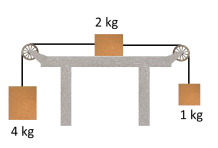
\includegraphics[width=0.48\textwidth]{ejercicio7_tres_masas.png}
\end{center}

Para distinguir las cuerdas, llamaremos $T_1$ a la tensión de la cuerda izquierda y $T_2$ a la tensión de la cuerda derecha.

\paso{1}{Definición del sistema en estudio}
Se analizan tres sistemas, uno para cada bloque:
\begin{itemize}[itemsep=2pt]
  \item bloque izquierdo: $m_1=\SI{4}{\kilogram}$;
  \item bloque central: $m_2=\SI{2}{\kilogram}$;
  \item bloque derecho: $m_3=\SI{1}{\kilogram}$.
\end{itemize}

Las dos cuerdas son inextensibles. Por lo tanto, mientras permanecen tensas, los tres bloques tienen aceleraciones de igual módulo.

Antes de escribir las ecuaciones conviene anticipar el sentido del movimiento: el peso de $m_1$ es mayor que el de $m_3$ y debe además vencer el rozamiento del bloque central. Verificaremos que el sistema efectivamente acelera con $m_1$ hacia abajo, $m_2$ hacia la izquierda y $m_3$ hacia arriba.

\paso{2}{Hipótesis simplificativas}
\begin{itemize}[itemsep=2pt]
  \item Tierra plana.
  \item Modelo de partícula para los tres bloques.
  \item Cuerdas ideales: masa despreciable e inextensibles.
  \item Poleas ideales: masa despreciable y sin rozamiento en sus ejes.
  \item La mesa es horizontal y rígida.
  \item El rozamiento entre el bloque central y la mesa es cinético, con $\mu_k=0,35$.
  \item Se desprecia el efecto del aire.
\end{itemize}

\paso{3}{Interacciones y pares de acción y reacción}
\textbf{Bloque de $\SI{4}{\kilogram}$:}
\begin{itemize}[itemsep=2pt]
  \item Tierra--bloque: peso $\vec P_1$ hacia abajo;
  \item cuerda izquierda--bloque: tensión $\vec T_1$ hacia arriba.
\end{itemize}

\textbf{Bloque de $\SI{2}{\kilogram}$:}
\begin{itemize}[itemsep=2pt]
  \item Tierra--bloque: peso $\vec P_2$;
  \item mesa--bloque: normal $\vec N$ y rozamiento cinético $\vec f_k$;
  \item cuerda izquierda--bloque: tensión $\vec T_1$ hacia la izquierda;
  \item cuerda derecha--bloque: tensión $\vec T_2$ hacia la derecha.
\end{itemize}

\textbf{Bloque de $\SI{1}{\kilogram}$:}
\begin{itemize}[itemsep=2pt]
  \item Tierra--bloque: peso $\vec P_3$ hacia abajo;
  \item cuerda derecha--bloque: tensión $\vec T_2$ hacia arriba.
\end{itemize}

Cada interacción tiene su correspondiente fuerza de reacción sobre el otro cuerpo. Esas fuerzas de reacción no se dibujan en el mismo diagrama de cuerpo libre.

\paso{4}{Modelo de partícula y diagramas vectoriales}
Como el movimiento esperado del bloque central es hacia la izquierda, el rozamiento cinético de la mesa sobre dicho bloque apunta hacia la derecha.

La normal sobre el bloque central vale
\[
N=m_2g=(2)(9,8)=\SI{19.6}{\newton},
\]
y por lo tanto
\[
f_k=\mu_kN=(0,35)(19,6)=\SI{6.86}{\newton}.
\]

\subsubsection*{a) Bloque de $\SI{4}{\kilogram}$}
\begin{center}
\begin{tikzpicture}[scale=1.05,>=Latex]
  \coordinate (O) at (0,0);
  \fill (O) circle (2.3pt);
  \node[right] at (0.1,0) {$m_1=\SI{4}{\kilogram}$};
  \draw[->,very thick,AzulFisica] (O) -- ++(90:2.0) node[right] {$\vec T_1$};
  \draw[->,very thick,RojoFuerza] (O) -- ++(-90:2.5) node[right] {$\vec P_1$};
  \draw[->,thick,dashed] (-0.35,-0.25) -- ++(-90:1.25) node[left] {$\vec a$};
\end{tikzpicture}
\end{center}

\subsubsection*{b) Bloque de $\SI{2}{\kilogram}$}
\begin{center}
\begin{tikzpicture}[scale=1.05,>=Latex]
  \coordinate (O) at (0,0);
  \fill (O) circle (2.3pt);
  \node[below right] at (0.1,-0.05) {$m_2=\SI{2}{\kilogram}$};
  \draw[->,thin,gray] (-3.2,0) -- (3.2,0) node[right] {$x$};
  \draw[->,thin,gray] (0,-2.4) -- (0,2.4) node[above] {$y$};
  \draw[->,very thick,AzulFisica] (O) -- ++(180:2.7) node[above] {$\vec T_1$};
  \draw[->,very thick,AzulFisica] (O) -- ++(0:1.8) node[above] {$\vec T_2$};
  \draw[->,very thick,VerdeRoz] (O) -- ++(0:2.75) node[below=2pt] {$\vec f_k$};
  \draw[->,very thick,AzulFisica] (O) -- ++(90:1.8) node[right] {$\vec N$};
  \draw[->,very thick,RojoFuerza] (O) -- ++(-90:1.8) node[right] {$\vec P_2$};
  \draw[->,thick,dashed] (-0.15,-1.15) -- ++(180:1.4) node[below] {$\vec a$};
\end{tikzpicture}
\end{center}

\subsubsection*{c) Bloque de $\SI{1}{\kilogram}$}
\begin{center}
\begin{tikzpicture}[scale=1.05,>=Latex]
  \coordinate (O) at (0,0);
  \fill (O) circle (2.3pt);
  \node[right] at (0.1,0) {$m_3=\SI{1}{\kilogram}$};
  \draw[->,very thick,AzulFisica] (O) -- ++(90:2.5) node[right] {$\vec T_2$};
  \draw[->,very thick,RojoFuerza] (O) -- ++(-90:1.8) node[right] {$\vec P_3$};
  \draw[->,thick,dashed] (-0.35,0.25) -- ++(90:1.25) node[left] {$\vec a$};
\end{tikzpicture}
\end{center}

\paso{5}{Planteo de la segunda ley de Newton}
Elegimos como sentidos positivos los sentidos del movimiento esperado: hacia abajo para $m_1$, hacia la izquierda para $m_2$ y hacia arriba para $m_3$.

Para $m_1$:
\[
m_1g-T_1=m_1a.
\tag{1}
\]

Para $m_2$:
\[
T_1-T_2-f_k=m_2a.
\tag{2}
\]

Para $m_3$:
\[
T_2-m_3g=m_3a.
\tag{3}
\]

Al sumar las tres ecuaciones se cancelan las tensiones internas:
\[
m_1g-m_3g-f_k=(m_1+m_2+m_3)a.
\]

\paso{6}{Resolución matemática e interpretación}
Sustituyendo los valores:
\[
a=\frac{(4)(9,8)-(1)(9,8)-6,86}{4+2+1}.
\]
Por lo tanto,
\[
\boxed{a=\SI{3.22}{\meter\per\second\squared}}.
\]

El signo positivo confirma el sentido supuesto. Así:
\begin{itemize}[itemsep=2pt]
  \item el bloque de $\SI{4}{\kilogram}$ acelera \textbf{hacia abajo};
  \item el bloque de $\SI{2}{\kilogram}$ acelera \textbf{hacia la izquierda};
  \item el bloque de $\SI{1}{\kilogram}$ acelera \textbf{hacia arriba}.
\end{itemize}

Para la tensión izquierda, de la ecuación (1):
\[
T_1=m_1(g-a)=4(9,8-3,22),
\]
\[
\boxed{T_1\approx\SI{26.3}{\newton}}.
\]

Para la tensión derecha, de la ecuación (3):
\[
T_2=m_3(g+a)=1(9,8+3,22),
\]
\[
\boxed{T_2\approx\SI{13.0}{\newton}}.
\]

\vspace{0.5em}
\begin{center}
\fcolorbox{AzulFisica}{AzulClaro}{%
\begin{minipage}{0.88\textwidth}
\textbf{Resultados del ejercicio 7}
\[
\boxed{
\begin{aligned}
a&=\SI{3.22}{\meter\per\second\squared},\\
T_1&\approx\SI{26.3}{\newton},\\
T_2&\approx\SI{13.0}{\newton}.
\end{aligned}}
\]
Direcciones: $4\,\mathrm{kg}$ hacia abajo, $2\,\mathrm{kg}$ hacia la izquierda y $1\,\mathrm{kg}$ hacia arriba.
\end{minipage}}
\end{center}

% ============================================================
% EJERCICIO 8
% ============================================================
\ejercicio{Tres bloques conectados: superficie horizontal y plano inclinado rugosos}

\subsection*{Enunciado}
Los tres bloques de la figura están conectados mediante cuerdas sin masa que pasan por poleas sin rozamiento. Las masas son $\SI{10}{\kilogram}$, $\SI{5}{\kilogram}$ y $\SI{3}{\kilogram}$. El bloque de $\SI{3}{\kilogram}$ se encuentra sobre un plano inclinado $25^\circ$.

La aceleración del sistema es
\[
a=\SI{2.35}{\meter\per\second\squared}
\]
hacia la izquierda para el bloque de $\SI{5}{\kilogram}$. Las superficies de apoyo son rugosas y se supone el mismo coeficiente de rozamiento cinético $\mu_k$ para los bloques de $\SI{5}{\kilogram}$ y $\SI{3}{\kilogram}$.

Determinar:
\begin{enumerate}[label=\alph*)]
  \item las tensiones en las dos cuerdas;
  \item el coeficiente de rozamiento cinético $\mu_k$.
\end{enumerate}

\begin{center}
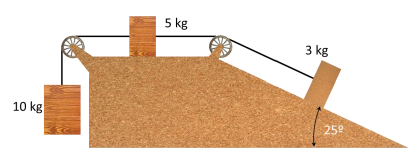
\includegraphics[width=0.55\textwidth]{ejercicio8_plano_inclinado.png}
\end{center}

Denominaremos $T_1$ a la tensión de la cuerda que une los bloques de $\SI{10}{\kilogram}$ y $\SI{5}{\kilogram}$, y $T_2$ a la tensión de la cuerda que une los bloques de $\SI{5}{\kilogram}$ y $\SI{3}{\kilogram}$.

\paso{1}{Definición del sistema en estudio}
Se analizan tres sistemas:
\begin{itemize}[itemsep=2pt]
  \item masa colgante $m_1=\SI{10}{\kilogram}$;
  \item bloque horizontal $m_2=\SI{5}{\kilogram}$;
  \item bloque sobre el plano inclinado $m_3=\SI{3}{\kilogram}$.
\end{itemize}

Como el bloque de $\SI{5}{\kilogram}$ acelera hacia la izquierda, las restricciones impuestas por las cuerdas indican que:
\begin{itemize}[itemsep=2pt]
  \item el bloque de $\SI{10}{\kilogram}$ acelera hacia abajo;
  \item el bloque de $\SI{3}{\kilogram}$ acelera hacia arriba del plano inclinado.
\end{itemize}
Los tres tienen aceleraciones de igual módulo, $a=\SI{2.35}{\meter\per\second\squared}$.

\paso{2}{Hipótesis simplificativas}
\begin{itemize}[itemsep=2pt]
  \item Tierra plana.
  \item Modelo de partícula para los tres bloques.
  \item Cuerdas ideales: masa despreciable e inextensibles.
  \item Poleas ideales: sin rozamiento y de masa despreciable.
  \item Superficies rígidas.
  \item El mismo coeficiente de rozamiento cinético $\mu_k$ actúa en la superficie horizontal y en el plano inclinado.
  \item Se desprecia el efecto del aire.
\end{itemize}

\paso{3}{Interacciones y pares de acción y reacción}
\textbf{Bloque de $\SI{10}{\kilogram}$:} peso $\vec P_1$ y tensión $\vec T_1$.

\textbf{Bloque de $\SI{5}{\kilogram}$:} peso $\vec P_2$, normal $\vec N_2$, tensiones $\vec T_1$ y $\vec T_2$, y rozamiento cinético $\vec f_{k2}$.

\textbf{Bloque de $\SI{3}{\kilogram}$:} peso $\vec P_3$, normal $\vec N_3$, tensión $\vec T_2$ y rozamiento cinético $\vec f_{k3}$.

El rozamiento siempre se opone al movimiento relativo entre las superficies. Por ello, sobre el bloque de $\SI{5}{\kilogram}$ apunta hacia la derecha, y sobre el bloque de $\SI{3}{\kilogram}$ apunta cuesta abajo.

\paso{4}{Modelo de partícula y diagramas vectoriales}

\subsubsection*{a) Masa colgante de $\SI{10}{\kilogram}$}
\begin{center}
\begin{tikzpicture}[scale=1.05,>=Latex]
  \coordinate (O) at (0,0);
  \fill (O) circle (2.3pt);
  \node[right] at (0.1,0) {$m_1=\SI{10}{\kilogram}$};
  \draw[->,very thick,AzulFisica] (O) -- ++(90:2.0) node[right] {$\vec T_1$};
  \draw[->,very thick,RojoFuerza] (O) -- ++(-90:2.7) node[right] {$\vec P_1$};
  \draw[->,thick,dashed] (-0.35,-0.25) -- ++(-90:1.25) node[left] {$\vec a$};
\end{tikzpicture}
\end{center}

\subsubsection*{b) Bloque de $\SI{5}{\kilogram}$ sobre la superficie horizontal}
\begin{center}
\begin{tikzpicture}[scale=1.05,>=Latex]
  \coordinate (O) at (0,0);
  \fill (O) circle (2.3pt);
  \node[below right] at (0.1,-0.05) {$m_2=\SI{5}{\kilogram}$};
  \draw[->,thin,gray] (-3.2,0) -- (3.2,0) node[right] {$x$};
  \draw[->,thin,gray] (0,-2.4) -- (0,2.4) node[above] {$y$};
  \draw[->,very thick,AzulFisica] (O) -- ++(180:2.65) node[above] {$\vec T_1$};
  \draw[->,very thick,AzulFisica] (O) -- ++(0:1.75) node[above] {$\vec T_2$};
  \draw[->,very thick,VerdeRoz] (O) -- ++(0:2.75) node[below=2pt] {$\vec f_{k2}$};
  \draw[->,very thick,AzulFisica] (O) -- ++(90:1.8) node[right] {$\vec N_2$};
  \draw[->,very thick,RojoFuerza] (O) -- ++(-90:1.8) node[right] {$\vec P_2$};
  \draw[->,thick,dashed] (-0.15,-1.15) -- ++(180:1.4) node[below] {$\vec a$};
\end{tikzpicture}
\end{center}

En la dirección vertical,
\[
N_2=m_2g=5g,
\]
por lo que
\[
f_{k2}=\mu_km_2g.
\]

\subsubsection*{c) Bloque de $\SI{3}{\kilogram}$ sobre el plano inclinado}
Para este bloque elegimos el eje $x'$ paralelo al plano, positivo cuesta arriba, y el eje $y'$ normal al plano.

\begin{center}
\begin{tikzpicture}[scale=1.08,>=Latex]
  \coordinate (O) at (0,0);
  \fill (O) circle (2.3pt);
  \node[below right] at (0.08,-0.05) {$m_3=\SI{3}{\kilogram}$};

  % ejes rotados: x' a 155 grados (cuesta arriba hacia la izquierda), y' normal a 65 grados
  \draw[->,thin,gray] (O) -- ++(155:3.2) node[above left] {$x'$};
  \draw[->,thin,gray] (O) -- ++(65:2.5) node[above] {$y'$};

  \draw[->,very thick,AzulFisica] (O) -- ++(155:2.7) node[above left] {$\vec T_2$};
  \draw[->,very thick,VerdeRoz] (O) -- ++(-25:2.1) node[below right] {$\vec f_{k3}$};
  \draw[->,very thick,AzulFisica] (O) -- ++(65:1.8) node[right] {$\vec N_3$};
  \draw[->,very thick,RojoFuerza] (O) -- ++(-90:2.2) node[right] {$\vec P_3$};
  \draw[->,thick,dashed] (-0.2,0.05) -- ++(155:1.35) node[below left] {$\vec a$};
\end{tikzpicture}
\end{center}

La componente del peso paralela al plano es
\[
P_{3\parallel}=m_3g\sin25^\circ,
\]
y la normal es
\[
N_3=m_3g\cos25^\circ.
\]
Por lo tanto,
\[
f_{k3}=\mu_km_3g\cos25^\circ.
\]

\paso{5}{Planteo de la segunda ley de Newton}
Elegimos como positivo el sentido de la aceleración de cada bloque.

\textbf{Bloque de $\SI{10}{\kilogram}$, positivo hacia abajo:}
\[
m_1g-T_1=m_1a.
\tag{1}
\]

\textbf{Bloque de $\SI{5}{\kilogram}$, positivo hacia la izquierda:}
\[
T_1-T_2-f_{k2}=m_2a,
\]
\[
T_1-T_2-\mu_km_2g=m_2a.
\tag{2}
\]

\textbf{Bloque de $\SI{3}{\kilogram}$, positivo cuesta arriba:}
\[
T_2-m_3g\sin25^\circ-f_{k3}=m_3a,
\]
\[
T_2-m_3g\sin25^\circ-\mu_km_3g\cos25^\circ=m_3a.
\tag{3}
\]

Las incógnitas son $T_1$, $T_2$ y $\mu_k$.

\paso{6}{Resolución matemática e interpretación}
De la ecuación (1):
\[
T_1=m_1(g-a)=10(9,8-2,35),
\]
\[
\boxed{T_1=\SI{74.5}{\newton}}.
\]

A partir de la ecuación (2):
\[
T_2=T_1-m_2a-\mu_km_2g.
\tag{4}
\]

De la ecuación (3):
\[
T_2=m_3a+m_3g\sin25^\circ+\mu_km_3g\cos25^\circ.
\tag{5}
\]

Igualando (4) y (5):
\[
T_1-m_2a-m_3a-m_3g\sin25^\circ
=\mu_k\left(m_2g+m_3g\cos25^\circ\right).
\]
Por lo tanto,
\[
\mu_k=
\frac{74,5-(5)(2,35)-(3)(2,35)-(3)(9,8)\sin25^\circ}
{(5)(9,8)+(3)(9,8)\cos25^\circ}.
\]
Así,
\[
\boxed{\mu_k\approx0,572}.
\]

Finalmente, sustituyendo este valor en cualquiera de las ecuaciones (4) o (5):
\[
T_2\approx\SI{34.7}{\newton}.
\]
Por lo tanto,
\[
\boxed{T_2\approx\SI{34.7}{\newton}}.
\]

\vspace{0.5em}
\begin{center}
\fcolorbox{AzulFisica}{AzulClaro}{%
\begin{minipage}{0.88\textwidth}
\textbf{Resultados del ejercicio 8}
\[
\boxed{
\begin{aligned}
T_1&=\SI{74.5}{\newton},\\
T_2&\approx\SI{34.7}{\newton},\\
\mu_k&\approx0,572.
\end{aligned}}
\]
\end{minipage}}
\end{center}

\textbf{Interpretación física.} La tensión izquierda es mayor porque la masa de $\SI{10}{\kilogram}$ es la principal fuerza motriz del sistema. El rozamiento sobre los bloques de $\SI{5}{\kilogram}$ y $\SI{3}{\kilogram}$ se opone a sus movimientos respectivos y reduce la aceleración hasta el valor dado de $\SI{2.35}{\meter\per\second\squared}$.


% ============================================================
% NUEVO BLOQUE TEMÁTICO: MOVIMIENTO CIRCULAR
% ============================================================
\clearpage
\section*{\color{AzulFisica}Ejercicios de movimiento circular}
\addcontentsline{toc}{section}{Ejercicios de movimiento circular}

En los ejercicios que siguen se aplicará la segunda ley de Newton a situaciones en las que la trayectoria es circular. La estrategia de resolución conserva los mismos seis pasos utilizados hasta aquí, pero resulta especialmente importante elegir una dirección \textbf{radial} orientada hacia el centro de la trayectoria.

Para movimiento circular, la componente radial de la segunda ley se expresa como
\[
\sum F_r = m a_r = m\frac{v^2}{r}.
\]

La llamada \emph{fuerza centrípeta} no es una fuerza adicional: es el nombre que recibe la \textbf{resultante de las componentes radiales de las fuerzas reales} que actúan sobre el sistema. Si la rapidez también cambia, será necesario analizar además la componente tangencial mediante
\[
\sum F_t = m a_t.
\]


% ============================================================
% EJERCICIO 9
% ============================================================
\ejercicio{Masa atada a una cuerda en un círculo vertical}

\subsection*{Enunciado}
Un pequeño bloque de masa $m=\SI{1}{\kilogram}$ está atado a una cuerda de longitud $r=\SI{0.6}{\meter}$ y gira a $60\ \text{rpm}$ en un círculo vertical. Calcular la tensión en la cuerda cuando el bloque está:
\begin{enumerate}[label=\alph*)]
  \item en el punto más alto del círculo;
  \item en el punto más bajo;
  \item cuando la cuerda está horizontal;
  \item y la velocidad lineal que debe tener en el punto más alto para que la tensión sea cero.
\end{enumerate}

\paso{1}{Definición del sistema en estudio}
El sistema en estudio es el \textbf{bloque de $\SI{1}{\kilogram}$}. Se analizará como partícula en tres posiciones de una trayectoria circular vertical: punto superior, punto inferior y punto lateral.

\paso{2}{Hipótesis simplificativas}
\begin{itemize}[itemsep=2pt]
  \item Tierra plana y campo gravitatorio uniforme.
  \item Modelo de partícula para el bloque.
  \item Cuerda ideal, de masa despreciable e inextensible.
  \item Se desprecia el efecto del aire.
  \item El radio de la trayectoria coincide con la longitud de la cuerda: $r=\SI{0.6}{\meter}$.
  \item Se interpreta el dato $60\ \text{rpm}$ como rapidez angular constante para los incisos a), b) y c).
\end{itemize}

La rapidez angular es
\[
\omega=60\frac{\text{rev}}{\text{min}}
\left(\frac{1\ \text{min}}{60\ \text{s}}\right)
(2\pi\ \text{rad/rev})=2\pi\ \text{rad/s}.
\]
Por lo tanto,
\[
v=\omega r=(2\pi)(0,6)=\SI{3.77}{\meter\per\second}.
\]

\paso{3}{Interacciones y pares de acción y reacción}
Sobre el bloque actúan únicamente:
\begin{itemize}[itemsep=2pt]
  \item la interacción \textbf{Tierra--bloque}, representada por el peso $\vec P=m\vec g$;
  \item la interacción \textbf{cuerda--bloque}, representada por la tensión $\vec T$, siempre dirigida a lo largo de la cuerda hacia el centro de la trayectoria.
\end{itemize}

Las fuerzas de reacción correspondientes actúan sobre la Tierra y sobre la cuerda, respectivamente, y no se incluyen en el diagrama de cuerpo libre del bloque.

\paso{4}{Modelo de partícula y diagramas vectoriales}
En movimiento circular resulta conveniente elegir en cada posición un eje radial positivo \textbf{hacia el centro}.

\begin{center}
\begin{tikzpicture}[scale=1.0,>=Latex]
  % Punto alto
  \begin{scope}[xshift=-5.0cm]
    \node[font=\bfseries] at (0,2.35) {Punto más alto};
    \fill (0,1.65) circle (2.5pt);
    \draw[dashed,gray,->] (0,1.45)--(0,-1.55);
    \draw[->,very thick,AzulFisica] (-0.10,1.62)--(-0.10,0.35) node[left] {$\vec T$};
    \draw[->,very thick,RojoFuerza] (0.10,1.62)--(0.10,-0.15) node[right] {$\vec P$};
  \end{scope}

  % Punto bajo
  \begin{scope}[xshift=0cm]
    \node[font=\bfseries] at (0,2.35) {Punto más bajo};
    \fill (0,0) circle (2.5pt);
    \draw[dashed,gray,->] (0,0.20)--(0,2.00);
    \draw[->,very thick,AzulFisica] (-0.10,0.03)--(-0.10,1.45) node[left] {$\vec T$};
    \draw[->,very thick,RojoFuerza] (0.10,-0.03)--(0.10,-1.40) node[right] {$\vec P$};
  \end{scope}

  % Cuerda horizontal
  \begin{scope}[xshift=5.0cm]
    \node[font=\bfseries] at (0,2.35) {Cuerda horizontal};
    \fill (0,0) circle (2.5pt);
    \draw[dashed,gray,->] (-0.20,0)--(-2.15,0);
    \draw[->,very thick,AzulFisica] (-0.03,0.08)--(-1.55,0.08) node[above] {$\vec T$};
    \draw[->,very thick,RojoFuerza] (0,-0.03)--(0,-1.45) node[right] {$\vec P$};
  \end{scope}
\end{tikzpicture}
\end{center}

\paso{5}{Planteo de la segunda ley de Newton}
La aceleración radial tiene módulo
\[
a_r=\frac{v^2}{r},
\]
y la resultante radial debe cumplir
\[
\sum F_r=m\frac{v^2}{r}.
\]
Con los datos:
\[
m\frac{v^2}{r}=1\frac{(3,77)^2}{0,6}\approx\SI{23.69}{\newton}.
\]

\textbf{Punto más alto:} tanto $T$ como $P$ apuntan hacia el centro,
\[
T+mg=m\frac{v^2}{r}.
\tag{1}
\]

\textbf{Punto más bajo:} $T$ apunta hacia el centro y el peso en sentido contrario,
\[
T-mg=m\frac{v^2}{r}.
\tag{2}
\]

\textbf{Cuerda horizontal:} el peso es perpendicular al radio, por lo que no tiene componente radial,
\[
T=m\frac{v^2}{r}.
\tag{3}
\]

Para el inciso d), en el punto más alto se impone $T=0$:
\[
mg=m\frac{v^2}{r}.
\tag{4}
\]

\paso{6}{Resolución matemática e interpretación}
\textbf{a) Punto más alto}
\[
T=\frac{mv^2}{r}-mg=23,69-9,8,
\]
\[
\boxed{T_{\text{alto}}\approx\SI{13.9}{\newton}}.
\]

\textbf{b) Punto más bajo}
\[
T=\frac{mv^2}{r}+mg=23,69+9,8,
\]
\[
\boxed{T_{\text{bajo}}\approx\SI{33.5}{\newton}}.
\]

\textbf{c) Cuerda horizontal}
\[
\boxed{T_{\text{horizontal}}\approx\SI{23.7}{\newton}}.
\]

\textbf{d) Tensión nula en el punto más alto}
\[
v=\sqrt{gr}=\sqrt{(9,8)(0,6)},
\]
\[
\boxed{v_{\min,\text{alto}}\approx\SI{2.42}{\meter\per\second}}.
\]

\begin{center}
\fcolorbox{AzulFisica}{AzulClaro}{%
\begin{minipage}{0.88\textwidth}
\textbf{Resultados del ejercicio 9}
\[
\boxed{
\begin{aligned}
T_{\text{alto}}&\approx\SI{13.9}{\newton},\\
T_{\text{bajo}}&\approx\SI{33.5}{\newton},\\
T_{\text{horizontal}}&\approx\SI{23.7}{\newton},\\
v_{\min,\text{alto}}&\approx\SI{2.42}{\meter\per\second}.
\end{aligned}}
\]
\end{minipage}}
\end{center}

\textbf{Interpretación física.} La tensión es máxima en el punto inferior porque allí debe producir la aceleración centrípeta y además compensar el peso. En el punto superior, el peso colabora con la tensión para producir la resultante radial.

% ============================================================
% EJERCICIO 10
% ============================================================
\ejercicio{Velocidad máxima antes de romper una cuerda}

\subsection*{Enunciado}
Una piedra de masa $m=\SI{1}{\kilogram}$ está atada al extremo de una cuerda de longitud $r=\SI{1}{\meter}$, cuya tensión de ruptura es $\SI{500}{\newton}$. La piedra gira describiendo una circunferencia sobre un tablero horizontal liso. El otro extremo de la cuerda permanece fijo. Hallar la máxima velocidad que puede alcanzar la piedra sin que se rompa la cuerda.

\paso{1}{Definición del sistema en estudio}
El sistema en estudio es la \textbf{piedra}, modelada como partícula que describe movimiento circular horizontal de radio $r=\SI{1}{\meter}$.

\paso{2}{Hipótesis simplificativas}
\begin{itemize}[itemsep=2pt]
  \item Tierra plana.
  \item Modelo de partícula.
  \item Cuerda ideal hasta alcanzar su tensión máxima admisible.
  \item Tablero horizontal liso: rozamiento despreciable.
  \item Se desprecia el efecto del aire.
  \item Movimiento circular uniforme en el instante límite considerado.
\end{itemize}

\paso{3}{Interacciones y pares de acción y reacción}
Sobre la piedra actúan:
\begin{itemize}[itemsep=2pt]
  \item peso $\vec P$ por interacción Tierra--piedra;
  \item normal $\vec N$ por interacción tablero--piedra;
  \item tensión $\vec T$ por interacción cuerda--piedra.
\end{itemize}
En vertical, $N$ y $P$ se equilibran. En horizontal, la tensión es la única fuerza radial.

\paso{4}{Modelo de partícula y diagrama vectorial}
\begin{center}
\begin{tikzpicture}[scale=1.05,>=Latex]
  \coordinate (C) at (-2.3,0);
  \coordinate (O) at (0,0);
  \draw[gray,dashed] (C) circle (2.3);
  \fill (C) circle (2pt) node[below] {punto fijo};
  \fill (O) circle (2.5pt) node[below right] {piedra};
  \draw[thick] (C)--(O);
  \draw[->,very thick,AzulFisica] (O)--(C) node[midway,above] {$\vec T$};
  \draw[->,very thick,AzulFisica] (O) -- ++(90:1.7) node[right] {$\vec N$};
  \draw[->,very thick,RojoFuerza] (O) -- ++(-90:1.7) node[right] {$\vec P$};
  \draw[->,thick,dashed] (O) -- ++(90:2.6) node[above] {$\vec v$};
\end{tikzpicture}
\end{center}

\paso{5}{Planteo de la segunda ley de Newton}
En la dirección vertical:
\[
N-mg=0.
\]
En la dirección radial horizontal:
\[
T=m\frac{v^2}{r}.
\]
En el límite antes de la ruptura,
\[
T=T_{\max}=\SI{500}{\newton}.
\]

\paso{6}{Resolución matemática e interpretación}
\[
v_{\max}=\sqrt{\frac{T_{\max}r}{m}}
=\sqrt{\frac{(500)(1)}{1}}.
\]
Por lo tanto,
\[
\boxed{v_{\max}\approx\SI{22.4}{\meter\per\second}}.
\]

La tensión crece proporcionalmente a $v^2$; por ello, un aumento relativamente pequeño de la rapidez cerca del límite puede provocar la ruptura de la cuerda.

% ============================================================
% EJERCICIO 11
% ============================================================
\ejercicio{Péndulo cónico}

\subsection*{Enunciado}
Considere un péndulo cónico con una plomada de masa $m=\SI{80}{\kilogram}$ suspendida de un alambre de longitud $L=\SI{10}{\meter}$ que forma un ángulo de $5^\circ$ con la vertical. Determinar:
\begin{enumerate}[label=\alph*)]
  \item las componentes horizontal y vertical de la fuerza ejercida por el alambre sobre la plomada;
  \item la aceleración radial de la plomada.
\end{enumerate}

\begin{center}
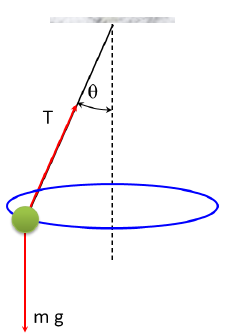
\includegraphics[width=0.34\textwidth]{ejercicio11_pendulo_conico.png}
\end{center}

\paso{1}{Definición del sistema en estudio}
El sistema es la \textbf{plomada de $\SI{80}{\kilogram}$}, considerada como partícula que describe una circunferencia horizontal. El centro de la trayectoria se encuentra sobre el eje vertical que pasa por el punto de suspensión.

\paso{2}{Hipótesis simplificativas}
\begin{itemize}[itemsep=2pt]
  \item Tierra plana y campo gravitatorio uniforme.
  \item Modelo de partícula para la plomada.
  \item Alambre ideal de masa despreciable e inextensible.
  \item Se desprecia el efecto del aire.
  \item Movimiento circular uniforme.
\end{itemize}

\paso{3}{Interacciones y pares de acción y reacción}
Sobre la plomada actúan dos fuerzas reales:
\begin{itemize}[itemsep=2pt]
  \item el peso $\vec P=m\vec g$, vertical hacia abajo;
  \item la tensión $\vec T$ ejercida por el alambre, dirigida a lo largo de éste hacia el punto de suspensión.
\end{itemize}
La componente vertical de $\vec T$ equilibra el peso y su componente horizontal proporciona la fuerza centrípeta.

\paso{4}{Modelo de partícula y diagrama vectorial}
\begin{center}
\begin{tikzpicture}[scale=1.15,>=Latex]
  \coordinate (O) at (0,0);
  \fill (O) circle (2.4pt) node[below right] {plomada};
  \draw[->,thin,gray] (0,-2.5)--(0,2.8) node[above] {vertical};
  \draw[->,thin,gray] (-0.15,0)--(-3.2,0) node[left] {radial hacia el centro};
  \draw[->,very thick,AzulFisica] (O)--++(95:3.0) node[above left] {$\vec T$};
  \draw[->,very thick,RojoFuerza] (O)--++(-90:2.1) node[right] {$\vec P$};
  \draw[->,very thick,AzulFisica!75] (O)--++(90:2.55) node[right] {$T\cos5^\circ$};
  \draw[->,very thick,AzulFisica!75] (O)--++(180:0.72) node[above] {$T\sin5^\circ$};
  \draw[dashed,gray] (0,0)--(0,2.7);
  \node at (-0.34,2.18) {$5^\circ$};
\end{tikzpicture}
\end{center}

\paso{5}{Planteo de la segunda ley de Newton}
En la dirección vertical no hay aceleración:
\[
T\cos5^\circ-mg=0.
\]
Por lo tanto, la componente vertical de la fuerza del alambre es
\[
T_y=T\cos5^\circ=mg.
\]
En la dirección radial:
\[
T\sin5^\circ=ma_r.
\]
Dividiendo ambas ecuaciones:
\[
\tan5^\circ=\frac{a_r}{g}.
\]

\paso{6}{Resolución matemática e interpretación}
La componente vertical es
\[
T_y=mg=(80)(9,8)=\SI{784}{\newton}.
\]
Así,
\[
\boxed{T_y=\SI{784}{\newton}}.
\]

La componente horizontal es
\[
T_x=T_y\tan5^\circ=(784)\tan5^\circ,
\]
\[
\boxed{T_x\approx\SI{68.6}{\newton}}.
\]

La aceleración radial resulta
\[
a_r=\frac{T_x}{m}=g\tan5^\circ,
\]
\[
\boxed{a_r\approx\SI{0.857}{\meter\per\second\squared}}.
\]

Como verificación, el módulo de la tensión es
\[
T=\frac{mg}{\cos5^\circ}\approx\SI{787}{\newton}.
\]

% ============================================================
% EJERCICIO 12
% ============================================================
\ejercicio{Automóvil en una curva horizontal plana}

\subsection*{Enunciado}
Un automóvil de masa $m=\SI{1500}{\kilogram}$ se mueve sobre un camino horizontal plano y recorre una curva de radio $r=\SI{35}{\meter}$. Si el coeficiente de fricción estática entre las llantas y el pavimento seco es $\mu_s=0,50$, encontrar la rapidez máxima que puede tener el automóvil para tomar la curva sin derrapar.

\begin{center}
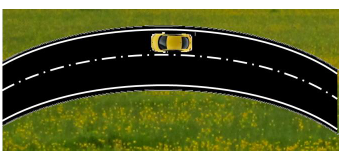
\includegraphics[width=0.62\textwidth]{ejercicio12_auto_curva.png}
\end{center}

\paso{1}{Definición del sistema en estudio}
El sistema es el \textbf{automóvil}, modelado como partícula que describe una trayectoria circular horizontal de radio $\SI{35}{\meter}$.

\paso{2}{Hipótesis simplificativas}
\begin{itemize}[itemsep=2pt]
  \item Tierra plana.
  \item Modelo de partícula para el automóvil.
  \item Carretera horizontal, sin peralte.
  \item El automóvil no desliza mientras $f_s\leq f_{s,\max}$.
  \item Se desprecia la resistencia del aire.
  \item Movimiento circular uniforme.
\end{itemize}

\paso{3}{Interacciones y pares de acción y reacción}
Sobre el automóvil actúan:
\begin{itemize}[itemsep=2pt]
  \item peso $\vec P$ hacia abajo;
  \item normal $\vec N$ del pavimento hacia arriba;
  \item rozamiento estático $\vec f_s$ horizontal hacia el centro de la curva.
\end{itemize}
La fuerza de rozamiento estático es, en este caso, la fuerza real que produce la aceleración centrípeta.

\paso{4}{Modelo de partícula y diagrama vectorial}
\begin{center}
\begin{tikzpicture}[scale=1.15,>=Latex]
  \coordinate (O) at (0,0);
  \fill (O) circle (2.4pt) node[below right] {automóvil};
  \draw[->,thin,gray] (-0.15,0)--(-3.35,0) node[left] {radial hacia el centro};
  \draw[->,thin,gray] (0,-2.4)--(0,2.4) node[above] {$y$};
  \draw[->,very thick,VerdeRoz] (O)--++(180:2.5) node[above] {$\vec f_s$};
  \draw[->,very thick,AzulFisica] (O)--++(90:1.8) node[right] {$\vec N$};
  \draw[->,very thick,RojoFuerza] (O)--++(-90:1.8) node[right] {$\vec P$};
\end{tikzpicture}
\end{center}

\paso{5}{Planteo de la segunda ley de Newton}
En vertical:
\[
N-mg=0
\qquad\Rightarrow\qquad
N=mg.
\]
En el límite de adherencia,
\[
f_{s,\max}=\mu_sN=\mu_smg.
\]
Esta fuerza debe proporcionar la aceleración centrípeta máxima:
\[
\mu_smg=m\frac{v_{\max}^2}{r}.
\]

\paso{6}{Resolución matemática e interpretación}
La masa se simplifica:
\[
v_{\max}=\sqrt{\mu_sgr}.
\]
Sustituyendo:
\[
v_{\max}=\sqrt{(0,50)(9,8)(35)}.
\]
Por lo tanto,
\[
\boxed{v_{\max}\approx\SI{13.1}{\meter\per\second}}.
\]
Equivalente a
\[
\boxed{v_{\max}\approx\SI{47.1}{\kilo\meter\per\hour}}.
\]

\textbf{Interpretación física.} La rapidez máxima no depende de la masa del vehículo porque tanto la fuerza de rozamiento máxima como la fuerza centrípeta requerida son proporcionales a $m$.

% ============================================================
% EJERCICIO 13
% ============================================================
\ejercicio{Peralte de una carretera sin necesidad de fricción lateral}

\subsection*{Enunciado}
Una carretera tiene un ancho de $\SI{13.6}{\meter}$. Calcular la diferencia de nivel entre los bordes exterior e interior para que un automóvil pueda viajar a $\SI{20}{\meter\per\second}$ por una curva de radio $R=\SI{600}{\meter}$ sin requerir fuerza lateral de rozamiento.

\paso{1}{Definición del sistema en estudio}
El sistema en estudio es el \textbf{automóvil} que recorre una curva peraltada. Se busca el ángulo de inclinación de la calzada para el cual no se necesita rozamiento lateral.

\paso{2}{Hipótesis simplificativas}
\begin{itemize}[itemsep=2pt]
  \item Tierra plana.
  \item Modelo de partícula para el automóvil.
  \item Curva circular de radio constante $R$.
  \item No se requiere fuerza de rozamiento lateral: $f=0$.
  \item Se desprecia el efecto del aire.
  \item Movimiento circular uniforme.
  \item El ancho $b=\SI{13.6}{\meter}$ se considera medido sobre la superficie inclinada de la carretera.
\end{itemize}

\paso{3}{Interacciones y pares de acción y reacción}
Sobre el automóvil actúan solamente:
\begin{itemize}[itemsep=2pt]
  \item el peso $\vec P=m\vec g$, vertical hacia abajo;
  \item la normal $\vec N$ de la carretera, perpendicular a la superficie.
\end{itemize}
La componente horizontal de $\vec N$ proporciona toda la fuerza centrípeta.

\paso{4}{Modelo de partícula y diagrama vectorial}
\begin{center}
\begin{tikzpicture}[scale=1.0,>=Latex]
  % Ángulo visual exagerado sólo para mejorar la lectura.
  \def\vang{18}

  % DCL a la izquierda
  \begin{scope}[xshift=-3.5cm]
    \node[font=\bfseries] at (0,2.35) {Modelo de partícula};
    \draw[very thick] (-1.5,{-1.5*tan(\vang)})--(1.5,{1.5*tan(\vang)});
    \coordinate (O) at (0,0);
    \fill (O) circle (2.4pt);
    \node[below right] at (O) {automóvil};
    \draw[->,very thick,RojoFuerza] (O)--++(-90:1.75) node[right] {$\vec P$};
    \draw[->,very thick,AzulFisica] (O)--++({90+\vang}:1.90) node[above left] {$\vec N$};
    \draw[->,thin,gray] (O)--++(180:2.35) node[left] {hacia el centro};
  \end{scope}

  % Geometría del peralte a la derecha
  \begin{scope}[xshift=3.8cm]
    \node[font=\bfseries] at (0,2.35) {Geometría del peralte};
    \coordinate (A) at (-2.2,-0.65);
    \coordinate (B) at (2.2,{4.4*tan(\vang)-0.65});
    \coordinate (H) at (2.2,-0.65);
    \draw[very thick] (A)--(B) node[midway,above,sloped] {$b=\SI{13.6}{\meter}$};
    \draw[dashed,gray] (A)--(H);
    \draw[<->,thick] (H)--(B) node[midway,right] {$h$};
    \node at (-1.45,-0.40) {$\theta$};
    \node[gray] at (0,-1.55) {esquema no a escala};
  \end{scope}
\end{tikzpicture}
\end{center}

\paso{5}{Planteo de la segunda ley de Newton}
Descomponiendo la normal:
\[
N\sin\theta=m\frac{v^2}{R},
\]
\[
N\cos\theta=mg.
\]
Dividiendo miembro a miembro:
\[
\tan\theta=\frac{v^2}{gR}.
\]
Geométricamente, si $b$ es el ancho medido sobre la superficie inclinada,
\[
h=b\sin\theta.
\]

\paso{6}{Resolución matemática e interpretación}
\[
\tan\theta=\frac{(20)^2}{(9,8)(600)}=0,0680.
\]
Por lo tanto,
\[
\theta\approx3,89^\circ.
\]
La diferencia de nivel es
\[
h=(13,6)\sin3,89^\circ,
\]
\[
\boxed{h\approx\SI{0.923}{\meter}}.
\]

Es decir, el borde exterior debe quedar aproximadamente
\[
\boxed{\SI{92.3}{\centi\meter}}
\]
por encima del borde interior.

\textbf{Interpretación física.} A la rapidez de diseño, la componente horizontal de la normal es suficiente para producir la aceleración centrípeta, de modo que el vehículo no necesita depender del rozamiento lateral.



% ============================================================
% NUEVO BLOQUE TEMATICO: MOVIMIENTO OSCILATORIO
% ============================================================
\clearpage
\section*{\color{AzulFisica}Ejercicios de movimiento oscilatorio}
\addcontentsline{toc}{section}{Ejercicios de movimiento oscilatorio}

En este bloque se conserva la estructura de seis pasos de la guía. En los problemas de movimiento armónico simple (MAS), el paso 5 se utiliza para formular las relaciones dinámicas y cinemáticas propias del modelo. Para pequeñas oscilaciones, la fuerza o el torque restaurador es proporcional y opuesto al desplazamiento respecto del equilibrio.

\[
F_x=-kx\qquad\Longrightarrow\qquad a_x=-\omega^2x,
\]
\[
\omega=\sqrt{\frac{k}{m}},\qquad
T=\frac{2\pi}{\omega},\qquad
f=\frac{1}{T}.
\]

% ============================================================
% EJERCICIO 14
% ============================================================
\ejercicio{Oscilador armónico descrito por su ecuación de posición}

\subsection*{Enunciado}
Un oscilador armónico simple está descrito por
\[
x=0,4\,\sen\!\left[\pi\left(0,1t+0,5\right)\right],
\]
donde $x$ y $t$ están expresados en metros y segundos, respectivamente. Hallar:
\begin{enumerate}[label=\alph*)]
  \item amplitud, periodo, frecuencia y fase inicial;
  \item expresiones generales para la velocidad y la aceleración;
  \item condiciones iniciales;
  \item posición, velocidad y aceleración para $t=\SI{5}{\second}$;
  \item representación de $x(t)$, $v(t)$ y $a(t)$.
\end{enumerate}

\paso{1}{Definición del sistema en estudio}
El sistema es una \textbf{partícula que oscila en una dimensión} alrededor de una posición de equilibrio que se toma como $x=0$. La ecuación dada especifica completamente su evolución temporal.

\paso{2}{Hipótesis simplificativas}
\begin{itemize}[itemsep=2pt]
  \item Modelo de partícula.
  \item Movimiento unidimensional.
  \item Oscilación armónica ideal, sin amortiguamiento ni fuerzas disipativas.
  \item La posición $x$ se mide desde el equilibrio.
  \item El tiempo $t=0$ se toma como origen temporal de la ecuación dada.
\end{itemize}

\paso{3}{Interacciones y pares de acción y reacción}
Para que el movimiento sea armónico simple debe existir una interacción restauradora cuya resultante sobre la partícula sea opuesta al desplazamiento. Si el oscilador se realiza con un resorte, la interacción resorte--partícula produce $\vec F_e=-k\vec x$, y la reacción correspondiente actúa sobre el resorte.

\paso{4}{Modelo de partícula y representación vectorial}
\begin{center}
\begin{tikzpicture}[>=Latex,scale=1.05]
  \draw[->,gray] (-4.3,0)--(4.3,0) node[right] {$x$};
  \draw[thick] (0,-0.18)--(0,0.18);
  \node[below] at (0,-0.18) {equilibrio};
  \coordinate (P) at (2.4,0);
  \fill (P) circle (2.5pt);
  \node[above] at (P) {partícula};
  \draw[->,very thick,RojoFuerza] (P)--++(180:1.65) node[above] {$\vec F_{\rm rest}$};
  \draw[<->,AzulFisica] (0,-0.75)--(2.4,-0.75) node[midway,below] {$x>0$};
  \node[align=center] at (0,-1.55) {La fuerza restauradora y la aceleración\\apuntan hacia el equilibrio.};
\end{tikzpicture}
\end{center}

\paso{5}{Planteo del modelo matemático del MAS}
La forma general adoptada es
\[
x=A\sen(\omega t+\phi_0).
\]
Comparando con la ecuación dada:
\[
x=0,4\sen(0,1\pi t+0,5\pi),
\]
se identifica
\[
A=\SI{0.4}{\meter},\qquad
\omega=0,1\pi\ \si{\radian\per\second},\qquad
\phi_0=\frac{\pi}{2}\ \si{\radian}.
\]
Las derivadas temporales son
\[
v(t)=\frac{dx}{dt}=A\omega\cos(\omega t+\phi_0),
\]
\[
a(t)=\frac{d^2x}{dt^2}=-A\omega^2\sen(\omega t+\phi_0)=-\omega^2x(t).
\]

\paso{6}{Resolución matemática e interpretación}
El periodo y la frecuencia son
\[
T=\frac{2\pi}{\omega}=\frac{2\pi}{0,1\pi}=\boxed{\SI{20}{\second}},
\qquad
f=\frac1T=\boxed{\SI{0.050}{\hertz}}.
\]
Por lo tanto,
\[
\boxed{v(t)=0,04\pi\cos(0,1\pi t+0,5\pi)\ \si{\meter\per\second}},
\]
\[
\boxed{a(t)=-0,004\pi^2\sen(0,1\pi t+0,5\pi)\ \si{\meter\per\second\squared}}.
\]

En $t=0$:
\[
x_0=\SI{0.4}{\meter},\qquad v_0=0,
\]
\[
a_0=-0,004\pi^2\approx\boxed{-\SI{0.0395}{\meter\per\second\squared}}.
\]
La partícula parte de la elongación positiva máxima y, por lo tanto, inicialmente se acelera hacia el equilibrio.

Para $t=\SI{5}{\second}$, el argumento vale $\pi$:
\[
\boxed{x(5)=0},
\]
\[
\boxed{v(5)=-0,04\pi\approx-\SI{0.126}{\meter\per\second}},
\]
\[
\boxed{a(5)=0}.
\]

\subsubsection*{Representación temporal}
\begin{center}
\begin{tikzpicture}[x=0.18cm,y=2.0cm,>=Latex]
  % x(t)
  \begin{scope}[yshift=3.6cm]
    \draw[->,gray] (0,0)--(42,0) node[right] {$t\,(\si{\second})$};
    \draw[->,gray] (0,-0.55)--(0,0.65) node[above] {$x\,(\si{\meter})$};
    \draw[AzulFisica,very thick,samples=180,domain=0:40,smooth,variable=\t]
      plot ({\t},{0.4*sin(deg(0.1*pi*\t+0.5*pi))});
    \foreach \t in {0,10,20,30,40} \draw (\t,0.03)--(\t,-0.03) node[below=2pt] {\small \t};
    \node[AzulFisica] at (34,0.48) {$x(t)$};
  \end{scope}
  % v(t), escala vertical grafica 1 unidad = 0.30 m/s
  \begin{scope}[yshift=1.7cm]
    \draw[->,gray] (0,0)--(42,0) node[right] {$t\,(\si{\second})$};
    \draw[->,gray] (0,-0.58)--(0,0.62) node[above] {$v$};
    \draw[VerdeRoz,very thick,samples=180,domain=0:40,smooth,variable=\t]
      plot ({\t},{3.1*0.04*pi*cos(deg(0.1*pi*\t+0.5*pi))});
    \node[VerdeRoz] at (34,0.46) {$v(t)$};
  \end{scope}
  % a(t), escala vertical grafica 1 unidad = 0.10 m/s2
  \begin{scope}[yshift=-0.2cm]
    \draw[->,gray] (0,0)--(42,0) node[right] {$t\,(\si{\second})$};
    \draw[->,gray] (0,-0.58)--(0,0.62) node[above] {$a$};
    \draw[RojoFuerza,very thick,samples=180,domain=0:40,smooth,variable=\t]
      plot ({\t},{12*(-0.004*pi*pi)*sin(deg(0.1*pi*\t+0.5*pi))});
    \node[RojoFuerza] at (34,0.46) {$a(t)$};
  \end{scope}
\end{tikzpicture}
\end{center}

\textbf{Interpretación física.} Posición y aceleración están en oposición de fase: $a=-\omega^2x$. La velocidad se desfasa un cuarto de periodo respecto de la posición y alcanza su módulo máximo al pasar por el equilibrio.

% ============================================================
% EJERCICIO 15
% ============================================================
\ejercicio{Periodo, frecuencia y frecuencia angular a partir del número de vibraciones}

\subsection*{Enunciado}
Un oscilador armónico simple tarda $\SI{12}{\second}$ en efectuar cinco vibraciones completas. Encontrar:
\begin{enumerate}[label=\alph*)]
  \item el periodo;
  \item la frecuencia en hertz;
  \item la frecuencia angular en radianes por segundo.
\end{enumerate}

\paso{1}{Definición del sistema en estudio}
El sistema es un oscilador que ejecuta un movimiento periódico. Se observa un intervalo de cinco ciclos completos.

\paso{2}{Hipótesis simplificativas}
\begin{itemize}[itemsep=2pt]
  \item Movimiento periódico estable.
  \item Cada ciclo tiene el mismo periodo.
  \item Se desprecia cualquier variación apreciable de la frecuencia durante los $\SI{12}{\second}$ observados.
\end{itemize}

\paso{3}{Interacciones y pares de acción y reacción}
El enunciado no especifica el mecanismo físico que produce la oscilación, por lo que no es necesario detallar fuerzas particulares. La información suministrada es puramente temporal.

\paso{4}{Modelo de partícula y representación del ciclo}
\begin{center}
\begin{tikzpicture}[>=Latex,scale=1.0]
  \draw[->,gray] (0,0)--(11.2,0) node[right] {$t$};
  \draw[AzulFisica,very thick,samples=160,domain=0:10.5,smooth,variable=\x]
    plot ({\x},{0.7*sin(deg(2*pi*\x/2.1))});
  \draw[<->,thick] (0,-1.2)--(10.5,-1.2) node[midway,below] {$5T=\SI{12}{\second}$};
  \node at (5.25,1.15) {cinco vibraciones completas};
\end{tikzpicture}
\end{center}

\paso{5}{Planteo de las relaciones periódicas}
Si en un tiempo $\Delta t$ se completan $N$ oscilaciones,
\[
T=\frac{\Delta t}{N},\qquad
f=\frac1T=\frac{N}{\Delta t},\qquad
\omega=2\pi f.
\]

\paso{6}{Resolución matemática e interpretación}
\[
T=\frac{12}{5}=\boxed{\SI{2.40}{\second}},
\]
\[
f=\frac{5}{12}=\boxed{\SI{0.417}{\hertz}},
\]
\[
\omega=2\pi\left(\frac{5}{12}\right)=\boxed{\SI{2.62}{\radian\per\second}}.
\]

\textbf{Interpretación física.} La frecuencia indica que el sistema realiza aproximadamente $0,417$ ciclos por segundo, mientras que $\omega$ expresa la rapidez de cambio de la fase en radianes por segundo.

% ============================================================
% EJERCICIO 16
% ============================================================
\ejercicio{MAS a partir de la aceleración máxima y la amplitud}

\subsection*{Enunciado}
Una partícula de masa $m=\SI{1}{\gram}$ vibra con movimiento armónico simple de amplitud $A=\SI{2}{\milli\meter}$. Su aceleración al final de la trayectoria es $a_{\max}=\SI{8.0e3}{\meter\per\second\squared}$. Calcular:
\begin{enumerate}[label=\alph*)]
  \item la frecuencia del movimiento;
  \item la velocidad de la partícula cuando pasa por el equilibrio y cuando $x=\SI{1.2}{\milli\meter}$;
  \item la fuerza que actúa sobre la partícula como función de la posición y como función del tiempo.
\end{enumerate}

\paso{1}{Definición del sistema en estudio}
El sistema en estudio es la partícula de
\[
m=\SI{0.001}{\kilogram}
\]
que oscila sobre un eje alrededor de $x=0$.

\paso{2}{Hipótesis simplificativas}
\begin{itemize}[itemsep=2pt]
  \item Modelo de partícula.
  \item MAS ideal y unidimensional.
  \item Se desprecia amortiguamiento.
  \item La aceleración indicada ``al final de la trayectoria'' se interpreta como su módulo máximo, correspondiente a $|x|=A$.
\end{itemize}

\paso{3}{Interacciones y pares de acción y reacción}
La interacción restauradora ejerce sobre la partícula una fuerza proporcional y opuesta al desplazamiento. La reacción de la partícula actúa sobre el elemento restaurador y no forma parte del DCL de la partícula.

\paso{4}{Modelo de partícula y diagrama vectorial}
\begin{center}
\begin{tikzpicture}[>=Latex,scale=1.05]
  \draw[->,gray] (-3.8,0)--(3.8,0) node[right] {$x$};
  \draw[thick] (0,-0.18)--(0,0.18) node[above=3pt] {equilibrio};
  \coordinate (P) at (2.4,0);
  \fill (P) circle (2.5pt);
  \draw[->,very thick,RojoFuerza] (P)--++(180:1.7) node[above] {$\vec F$};
  \draw[<->,AzulFisica] (0,-0.65)--(2.4,-0.65) node[midway,below] {$x$};
  \node[below] at (-3.1,-0.1) {$-A$};
  \node[below] at (3.1,-0.1) {$+A$};
\end{tikzpicture}
\end{center}

\paso{5}{Planteo de la segunda ley de Newton para el MAS}
En MAS,
\[
a=-\omega^2x.
\]
En un extremo, $|x|=A$, por lo que
\[
a_{\max}=\omega^2A.
\]
Además,
\[
v^2=\omega^2(A^2-x^2),
\]
y por la segunda ley,
\[
F=ma=-m\omega^2x.
\]

\paso{6}{Resolución matemática e interpretación}
Con $A=\SI{0.002}{\meter}$,
\[
\omega=\sqrt{\frac{8000}{0,002}}=\boxed{\SI{2000}{\radian\per\second}}.
\]
Entonces,
\[
f=\frac{\omega}{2\pi}=\boxed{\SI{318}{\hertz}}.
\]

En el equilibrio, $x=0$:
\[
v_{\max}=\omega A=(2000)(0,002)=\boxed{\SI{4.00}{\meter\per\second}}.
\]
Para $x=\SI{1.2}{\milli\meter}=\SI{0.0012}{\meter}$:
\[
|v|=2000\sqrt{(0,002)^2-(0,0012)^2}=\boxed{\SI{3.20}{\meter\per\second}}.
\]
El signo de $v$ dependerá del sentido en que la partícula atraviese esa posición.

La fuerza en función de $x$ es
\[
F(x)=-(0,001)(2000)^2x,
\]
\[
\boxed{F(x)=-4000x\ \si{\newton}},
\]
con $x$ expresado en metros.

Para escribir $F(t)$ es necesario fijar una fase. Tomando $t=0$ cuando la partícula se encuentra en $x=+A$,
\[
x(t)=A\cos(\omega t)=0,002\cos(2000t),
\]
por lo tanto
\[
\boxed{F(t)=-8\cos(2000t)\ \si{\newton}}.
\]
Una elección distinta del origen temporal modifica únicamente la fase, no la amplitud ni la frecuencia de la fuerza.

% ============================================================
% EJERCICIO 17
% ============================================================
\ejercicio{Masa suspendida de un resorte: constante elástica y periodo}

\subsection*{Enunciado}
Una partícula de $\SI{2}{\kilogram}$ suspendida de un resorte de masa despreciable produce en éste un alargamiento de $\SI{20}{\centi\meter}$.
\begin{enumerate}[label=\alph*)]
  \item ¿Cuál es la constante recuperadora del resorte?
  \item ¿Cuál es el periodo de vibración de la partícula de $\SI{2}{\kilogram}$?
  \item ¿Cuál sería el periodo de una partícula de $\SI{4}{\kilogram}$ pendiente del mismo resorte?
\end{enumerate}

\paso{1}{Definición del sistema en estudio}
Primero se estudia la masa de $\SI{2}{\kilogram}$ en su posición de equilibrio estático para determinar $k$. Luego se analiza la oscilación vertical alrededor de esa posición de equilibrio.

\paso{2}{Hipótesis simplificativas}
\begin{itemize}[itemsep=2pt]
  \item Modelo de partícula para la masa.
  \item Resorte ideal, de masa despreciable y que cumple la ley de Hooke.
  \item Tierra plana y $g=\SI{9.8}{\meter\per\second\squared}$.
  \item Oscilaciones dentro del régimen elástico y sin amortiguamiento.
  \item Se desprecia el efecto del aire.
\end{itemize}

\paso{3}{Interacciones y pares de acción y reacción}
Sobre la masa actúan la interacción gravitatoria Tierra--masa y la interacción elástica resorte--masa. El resorte ejerce una fuerza hacia arriba en el equilibrio, y la masa ejerce sobre el resorte una fuerza igual y opuesta.

\paso{4}{Modelo de partícula y diagrama de cuerpo libre}
\begin{center}
\begin{tikzpicture}[>=Latex,scale=1.0]
  \draw[very thick] (-1.6,2.8)--(1.6,2.8);
  \draw[thick,decorate,decoration={zigzag,segment length=5pt,amplitude=3pt}] (0,2.8)--(0,0.45);
  \fill (0,0) circle (2.5pt);
  \node[right] at (0.15,0) {$m$};
  \draw[->,very thick,AzulFisica] (0,0)--(0,1.45) node[right] {$\vec F_e$};
  \draw[->,very thick,RojoFuerza] (0,0)--(0,-1.45) node[right] {$\vec P$};
  \draw[<->,gray] (1.25,2.25)--(1.25,0.45) node[midway,right] {$\Delta L$};
\end{tikzpicture}
\end{center}

\paso{5}{Planteo de la segunda ley de Newton}
En equilibrio estático,
\[
\sum F_y=0\qquad\Rightarrow\qquad k\Delta L-mg=0.
\]
Así,
\[
k=\frac{mg}{\Delta L}.
\]
Para pequeñas oscilaciones verticales alrededor del equilibrio,
\[
T=2\pi\sqrt{\frac{m}{k}}.
\]

\paso{6}{Resolución matemática e interpretación}
\[
k=\frac{(2)(9,8)}{0,20}=\boxed{\SI{98}{\newton\per\meter}}.
\]
Para $m=\SI{2}{\kilogram}$:
\[
T_2=2\pi\sqrt{\frac{2}{98}}=\boxed{\SI{0.898}{\second}}.
\]
Para $m=\SI{4}{\kilogram}$:
\[
T_4=2\pi\sqrt{\frac{4}{98}}=\boxed{\SI{1.27}{\second}}.
\]

\textbf{Interpretación física.} Al utilizar el mismo resorte, duplicar la masa no duplica el periodo: éste aumenta en un factor $\sqrt{2}$.

% ============================================================
% EJERCICIO 18
% ============================================================
\ejercicio{Cambio del periodo de un péndulo al modificar su longitud}

\subsection*{Enunciado}
El periodo de un péndulo es $T_0=\SI{3}{\second}$. Calcular su nuevo periodo si:
\begin{enumerate}[label=\alph*)]
  \item su longitud aumenta un $60\%$;
  \item su longitud disminuye un $60\%$.
\end{enumerate}

\paso{1}{Definición del sistema en estudio}
El sistema es un péndulo simple que oscila con pequeña amplitud bajo el mismo campo gravitatorio antes y después de modificar su longitud.

\paso{2}{Hipótesis simplificativas}
\begin{itemize}[itemsep=2pt]
  \item Masa puntual suspendida de una cuerda ideal.
  \item Oscilaciones de pequeña amplitud: $\sen\theta\approx\theta$.
  \item La aceleración gravitatoria permanece constante.
  \item Se desprecia la resistencia del aire.
\end{itemize}

\paso{3}{Interacciones y pares de acción y reacción}
Sobre la masa actúan el peso y la tensión de la cuerda. La componente tangencial del peso es la responsable del movimiento restaurador. Las reacciones correspondientes actúan sobre la Tierra y sobre la cuerda, respectivamente.

\paso{4}{Modelo de partícula y diagrama vectorial}
\begin{center}
\begin{tikzpicture}[>=Latex,scale=1.05]
  \coordinate (O) at (0,2.5);
  \coordinate (P) at (1.35,0.25);
  \fill (O) circle (2.2pt);
  \draw[thick] (O)--(P);
  \fill (P) circle (2.7pt);
  \draw[dashed,gray] (O)--(0,-0.15);
  \draw[->,very thick,RojoFuerza] (P)--++(-90:1.65) node[right] {$\vec P$};
  \draw[->,very thick,AzulFisica] (P)--($(P)!0.64!(O)$) node[midway,right] {$\vec T$};
  \node at (0.34,1.75) {$\theta$};
  \node[right] at (0.72,1.35) {$L$};
\end{tikzpicture}
\end{center}

\paso{5}{Planteo del modelo del péndulo simple}
Para pequeñas oscilaciones,
\[
T=2\pi\sqrt{\frac{L}{g}}.
\]
Si $g$ no cambia, entre dos configuraciones se cumple
\[
\frac{T'}{T_0}=\sqrt{\frac{L'}{L_0}}.
\]

\paso{6}{Resolución matemática e interpretación}
Si la longitud aumenta un $60\%$,
\[
L'=1,60L_0,
\]
\[
T'=3\sqrt{1,60}=\boxed{\SI{3.79}{\second}}.
\]
Si la longitud disminuye un $60\%$,
\[
L'=0,40L_0,
\]
\[
T'=3\sqrt{0,40}=\boxed{\SI{1.90}{\second}}.
\]

\textbf{Interpretación física.} El periodo depende de la raíz cuadrada de la longitud; por eso cambios porcentuales grandes de $L$ producen cambios más moderados en $T$.

% ============================================================
% EJERCICIO 19
% ============================================================
\ejercicio{Péndulo simple en sistemas acelerados}

\subsection*{Enunciado}
Un péndulo simple mide $L=\SI{5}{\meter}$ de largo.
\begin{enumerate}[label=\alph*)]
  \item ¿Cuál es el periodo de pequeñas oscilaciones si se ubica en un elevador que acelera hacia arriba a $\SI{5.0}{\meter\per\second\squared}$?
  \item ¿Cuál es el periodo si el elevador acelera hacia abajo a $\SI{5.0}{\meter\per\second\squared}$?
  \item ¿Cuál es el periodo si el péndulo se coloca en un vehículo que acelera horizontalmente a $\SI{5.0}{\meter\per\second\squared}$?
\end{enumerate}

\textbf{Nota de edición.} En el archivo adjunto el inciso c) aparece truncado. Se completa con la formulación del mismo problema: vehículo con aceleración horizontal de $\SI{5.0}{\meter\per\second\squared}$. Asimismo, en el inciso a) se interpreta la unidad de la aceleración como $\si{\meter\per\second\squared}$.

\paso{1}{Definición del sistema en estudio}
El sistema es la masa del péndulo observada desde el marco solidario con el elevador o con el vehículo. Se estudian pequeñas oscilaciones alrededor de la nueva posición de equilibrio.

\paso{2}{Hipótesis simplificativas}
\begin{itemize}[itemsep=2pt]
  \item Péndulo simple: masa puntual y cuerda ideal inextensible.
  \item Oscilaciones pequeñas.
  \item Aceleración del elevador o del vehículo constante.
  \item $g=\SI{9.8}{\meter\per\second\squared}$.
  \item Se desprecia el aire.
\end{itemize}

\paso{3}{Interacciones y pares de acción y reacción}
Las fuerzas reales sobre la masa son el peso y la tensión. Al describir el problema desde un marco acelerado puede introducirse una fuerza inercial $-m\vec a_0$; ésta no es una interacción adicional, sino un recurso del marco no inercial. El efecto conjunto se expresa mediante una gravedad efectiva $\vec g_{\rm ef}=\vec g-\vec a_0$.

\paso{4}{Modelo de partícula y gravedad efectiva}
\begin{center}
\begin{tikzpicture}[>=Latex,scale=0.92]
  \begin{scope}[xshift=-5.0cm]
    \node[font=\bfseries] at (0,2.5) {Elevador: $\vec a_0\uparrow$};
    \fill (0,0.4) circle (2.5pt);
    \draw[->,very thick,RojoFuerza] (0,0.4)--(0,-1.45) node[right] {$m\vec g$};
    \draw[->,very thick,AzulFisica] (0,0.4)--(0,2.0) node[right] {$\vec T$};
    \draw[->,thick,VerdeRoz] (1.25,0.5)--(1.25,1.75) node[right] {$\vec a_0$};
    \node at (0,-2.0) {$g_{\rm ef}=g+a_0$};
  \end{scope}
  \begin{scope}
    \node[font=\bfseries] at (0,2.5) {Elevador: $\vec a_0\downarrow$};
    \fill (0,0.4) circle (2.5pt);
    \draw[->,very thick,RojoFuerza] (0,0.4)--(0,-1.45) node[right] {$m\vec g$};
    \draw[->,very thick,AzulFisica] (0,0.4)--(0,2.0) node[right] {$\vec T$};
    \draw[->,thick,VerdeRoz] (1.25,1.7)--(1.25,0.55) node[right] {$\vec a_0$};
    \node at (0,-2.0) {$g_{\rm ef}=g-a_0$};
  \end{scope}
  \begin{scope}[xshift=5.0cm]
    \node[font=\bfseries] at (0,2.5) {Vehículo: $\vec a_0\rightarrow$};
    \coordinate (B) at (0,0.4);
    \fill (B) circle (2.5pt);
    \draw[->,very thick,RojoFuerza] (B)--++(-90:1.55) node[right] {$m\vec g$};
    \draw[->,thick,VerdeRoz] (B)--++(180:1.25) node[above] {$-m\vec a_0$};
    \draw[->,very thick,AzulFisica] (B)--++(63:1.75) node[above] {$\vec T$};
    \draw[->,very thick,gray] (B)--++(244:1.95) node[below left] {$\vec g_{\rm ef}$};
  \end{scope}
\end{tikzpicture}
\end{center}

\paso{5}{Planteo del modelo dinámico}
Para pequeñas oscilaciones en un campo efectivo uniforme,
\[
T=2\pi\sqrt{\frac{L}{g_{\rm ef}}}.
\]
En los casos verticales:
\[
g_{\rm ef}=g+a_0\quad\text{(aceleración hacia arriba)},
\]
\[
g_{\rm ef}=g-a_0\quad\text{(aceleración hacia abajo)}.
\]
Para aceleración horizontal,
\[
g_{\rm ef}=\sqrt{g^2+a_0^2}.
\]

\paso{6}{Resolución matemática e interpretación}
\textbf{a) Elevador acelerando hacia arriba}
\[
g_{\rm ef}=9,8+5,0=\SI{14.8}{\meter\per\second\squared},
\]
\[
\boxed{T_{\uparrow}=2\pi\sqrt{\frac{5}{14,8}}=\SI{3.65}{\second}}.
\]

\textbf{b) Elevador acelerando hacia abajo}
\[
g_{\rm ef}=9,8-5,0=\SI{4.8}{\meter\per\second\squared},
\]
\[
\boxed{T_{\downarrow}=2\pi\sqrt{\frac{5}{4,8}}=\SI{6.41}{\second}}.
\]

\textbf{c) Vehículo acelerando horizontalmente}
\[
g_{\rm ef}=\sqrt{(9,8)^2+(5,0)^2}=\SI{11.00}{\meter\per\second\squared},
\]
\[
\boxed{T_h=2\pi\sqrt{\frac{5}{11,00}}=\SI{4.24}{\second}}.
\]
La nueva vertical efectiva se inclina un ángulo
\[
\theta=\tan^{-1}\!\left(\frac{5,0}{9,8}\right)\approx27,0^\circ
\]
respecto de la vertical gravitatoria.

% ============================================================
% NUEVO BLOQUE TEMATICO: CANTIDAD DE MOVIMIENTO
% ============================================================
\clearpage
\section*{\color{AzulFisica}Ejercicios de sistemas de partículas y cantidad de movimiento}
\addcontentsline{toc}{section}{Ejercicios de sistemas de partículas y cantidad de movimiento}

En estos problemas se mantiene el análisis de sistema e interacciones, pero el paso 5 se expresa mediante el teorema impulso--cantidad de movimiento o la conservación de la cantidad de movimiento del sistema cuando la resultante de impulsos externos es nula o despreciable.

\[
\vec J=\Delta\vec p,\qquad
\vec p=m\vec v,\qquad
\vec p_{\rm inicial}=\vec p_{\rm final}\quad(\vec J_{\rm ext}=0).
\]

% ============================================================
% EJERCICIO 20
% ============================================================
\ejercicio{Impulso sobre una pelota de béisbol}

\subsection*{Enunciado}
Una pelota de béisbol tiene una masa de $\SI{150}{\gram}$. Su velocidad antes del golpe es $\SI{24}{\meter\per\second}$ y, después de ser bateada, pasa a $\SI{36}{\meter\per\second}$ en sentido opuesto.
\begin{enumerate}[label=\alph*)]
  \item Calcular el incremento de su cantidad de movimiento y el impulso del golpe.
  \item Si permanece en contacto con el bate durante $\SI{0.002}{\second}$, hallar la fuerza media del golpe.
\end{enumerate}

\textbf{Nota de interpretación.} El archivo adjunto dice que la pelota ``pesa $150\ \mathrm{g}$''. Como el gramo es unidad de masa, se utiliza $m=\SI{150}{\gram}=\SI{0.150}{\kilogram}$.

\paso{1}{Definición del sistema en estudio}
El sistema es la \textbf{pelota} durante el intervalo de impacto con el bate. Elegimos como $+x$ el sentido de la velocidad inicial.

\paso{2}{Hipótesis simplificativas}
\begin{itemize}[itemsep=2pt]
  \item Modelo de partícula para la pelota.
  \item El intervalo de contacto es muy breve.
  \item Durante el choque, el impulso del peso y del aire es despreciable frente al impulso del bate.
  \item Movimiento analizado sobre el eje de la velocidad antes y después del impacto.
\end{itemize}

\paso{3}{Interacciones y pares de acción y reacción}
Durante el impacto la interacción dominante es bate--pelota. El bate ejerce una fuerza sobre la pelota y la pelota ejerce simultáneamente sobre el bate una fuerza igual y opuesta. Ambas actúan sobre cuerpos diferentes.

\paso{4}{Modelo de partícula y diagrama vectorial}
\begin{center}
\begin{tikzpicture}[>=Latex,scale=1.0]
  \node[font=\bfseries] at (-3.8,1.4) {Antes};
  \fill (-3.8,0) circle (3pt);
  \draw[->,very thick,AzulFisica] (-3.8,0)--(-0.9,0) node[midway,above] {$\vec v_i=+24$};
  \node[font=\bfseries] at (3.5,1.4) {Después};
  \fill (3.5,0) circle (3pt);
  \draw[->,very thick,RojoFuerza] (3.5,0)--(-0.3,0) node[midway,below] {$\vec v_f=-36$};
  \draw[->,gray] (-5.0,-1.15)--(5.0,-1.15) node[right] {$+x$};
\end{tikzpicture}
\end{center}

\paso{5}{Planteo del teorema impulso--cantidad de movimiento}
\[
\Delta p_x=m(v_f-v_i),
\]
\[
J_x=\Delta p_x.
\]
Si se usa una fuerza media durante el impacto,
\[
F_{\rm med}\,\Delta t=\Delta p_x.
\]

\paso{6}{Resolución matemática e interpretación}
Tomando $v_i=+\SI{24}{\meter\per\second}$ y $v_f=-\SI{36}{\meter\per\second}$:
\[
\Delta p_x=(0,150)(-36-24)=-\SI{9.0}{\kilogram\meter\per\second}.
\]
Por lo tanto,
\[
\boxed{\vec J=-9,0\,\hat\imath\ \si{\newton\second}}.
\]
El módulo del cambio de cantidad de movimiento y del impulso es $\SI{9.0}{\newton\second}$, dirigido en sentido opuesto a la velocidad inicial.

La fuerza media resulta
\[
F_{\rm med}=\frac{-9,0}{0,002}=-\SI{4.50e3}{\newton}.
\]
\[
\boxed{|F_{\rm med}|=\SI{4.50}{\kilo\newton}}.
\]

% ============================================================
% EJERCICIO 21
% ============================================================
\ejercicio{Muchacha caminando sobre un tablón sin rozamiento con el hielo}

\subsection*{Enunciado}
Una muchacha de $\SI{45}{\kilogram}$ está parada sobre un tablón de $\SI{150}{\kilogram}$. El tablón, inicialmente en reposo, puede deslizarse libremente sobre un lago congelado sin fricción. La muchacha camina a $\SI{1.5}{\meter\per\second}$ \textbf{respecto del tablón}. Determinar:
\begin{enumerate}[label=\alph*)]
  \item su velocidad respecto del hielo;
  \item la velocidad del tablón respecto del hielo.
\end{enumerate}

\paso{1}{Definición del sistema en estudio}
El sistema elegido para aplicar conservación de la cantidad de movimiento es \textbf{muchacha + tablón}. Para relacionar velocidades se distinguen el marco del hielo y el marco del tablón.

\paso{2}{Hipótesis simplificativas}
\begin{itemize}[itemsep=2pt]
  \item Tierra plana.
  \item El hielo es horizontal y sin fricción.
  \item Se desprecia el aire.
  \item El sistema parte del reposo.
  \item Las velocidades son horizontales.
\end{itemize}

\paso{3}{Interacciones y pares de acción y reacción}
La muchacha y el tablón se ejercen fuerzas de rozamiento estático internas, iguales y opuestas. Sobre el sistema completo no existe fuerza externa horizontal apreciable; peso y normales son verticales.

\paso{4}{Modelo del sistema y diagrama vectorial}
\begin{center}
\begin{tikzpicture}[>=Latex,scale=1.0]
  \draw[very thick] (-3.8,0)--(3.8,0);
  \draw[fill=AzulClaro,thick] (-2.5,0.05) rectangle (2.5,0.45);
  \fill (0,1.15) circle (2.8pt);
  \draw[thick] (0,1.1)--(0,0.55);
  \draw[thick] (0,0.85)--(-0.35,0.55);
  \draw[thick] (0,0.85)--(0.35,0.55);
  \node[above] at (0,1.25) {$m=45\ \mathrm{kg}$};
  \node[below] at (0,0.05) {$M=150\ \mathrm{kg}$};
  \draw[->,very thick,AzulFisica] (0.5,1.1)--(2.7,1.1) node[midway,above] {$v_m$};
  \draw[->,very thick,RojoFuerza] (-0.4,-0.4)--(-2.5,-0.4) node[midway,below] {$v_T$};
  \node at (0,-1.1) {$v_{m/T}=v_m-v_T=\SI{1.5}{\meter\per\second}$};
\end{tikzpicture}
\end{center}

\paso{5}{Planteo de conservación de cantidad de movimiento}
Como $p_{x,0}=0$ y $J_{x,\rm ext}=0$,
\[
m v_m+M v_T=0.
\]
La velocidad relativa dada es
\[
v_{m/T}=v_m-v_T=1,5.
\]

\paso{6}{Resolución matemática e interpretación}
De la conservación:
\[
v_T=-\frac{m}{M}v_m=-\frac{45}{150}v_m=-0,3v_m.
\]
Sustituyendo en la relación de velocidades:
\[
v_m-(-0,3v_m)=1,5,
\]
\[
1,3v_m=1,5.
\]
Por lo tanto,
\[
\boxed{v_m=\SI{1.15}{\meter\per\second}}
\]
respecto del hielo, en el sentido en que camina la muchacha, y
\[
\boxed{v_T=-\SI{0.346}{\meter\per\second}}
\]
respecto del hielo, es decir, en sentido contrario.

\textbf{Interpretación física.} El centro de masa del sistema permanece en reposo horizontalmente. El tablón retrocede para compensar la cantidad de movimiento adquirida por la muchacha.

% ============================================================
% NUEVO BLOQUE TEMATICO: CUERPO RIGIDO
% ============================================================
\clearpage
\section*{\color{AzulFisica}Ejercicios de cuerpo rígido}
\addcontentsline{toc}{section}{Ejercicios de cuerpo rígido}

Para un cuerpo rígido aparecen dos extensiones fundamentales del marco de resolución:
\[
I=\sum_i m_i r_i^2,\qquad
\sum\tau=I\alpha,
\]
y, cuando el cuerpo está en equilibrio,
\[
\sum\vec F=\vec 0,\qquad \sum\tau=0.
\]

% ============================================================
% EJERCICIO 22
% ============================================================
\ejercicio{Cuatro masas puntuales en los vértices de un rectángulo}

\subsection*{Enunciado}
Cuatro masas puntuales de $\SI{2}{\kilogram}$ están situadas en las esquinas de un rectángulo de $\SI{3}{\meter}\times\SI{2}{\meter}$.
\begin{enumerate}[label=\alph*)]
  \item Hallar el momento de inercia alrededor de un eje perpendicular al plano y que pasa por una de las masas.
  \item Si el sistema gira alrededor de ese eje con energía cinética rotacional de $\SI{184}{\joule}$, hallar el número de revoluciones por minuto.
\end{enumerate}

\paso{1}{Definición del sistema en estudio}
El sistema está constituido por las cuatro masas puntuales. El eje de rotación es perpendicular al plano del rectángulo y pasa por uno de los vértices.

\paso{2}{Hipótesis simplificativas}
\begin{itemize}[itemsep=2pt]
  \item Masas puntuales de $\SI{2}{\kilogram}$.
  \item Las uniones que mantienen la geometría del rectángulo se consideran rígidas y de masa despreciable.
  \item El eje es fijo y no tiene rozamiento apreciable.
\end{itemize}

\paso{3}{Interacciones y pares de acción y reacción}
Las fuerzas internas mantienen las separaciones entre las masas, pero no intervienen en el cálculo de $I$ respecto del eje especificado. Las reacciones del eje sostienen el sistema y, al ser un eje fijo ideal, no realizan trabajo rotacional neto.

\paso{4}{Modelo de sistema de partículas}
\begin{center}
\begin{tikzpicture}[>=Latex,scale=1.05]
  \coordinate (A) at (0,0);
  \coordinate (B) at (4.5,0);
  \coordinate (C) at (4.5,3.0);
  \coordinate (D) at (0,3.0);
  \draw[thick] (A)--(B)--(C)--(D)--cycle;
  \foreach \P in {A,B,C,D} \fill (\P) circle (3.3pt);
  \node[below left] at (A) {$m$};
  \node[below right] at (B) {$m$};
  \node[above right] at (C) {$m$};
  \node[above left] at (D) {$m$};
  \draw[<->,gray] (0,-0.65)--(4.5,-0.65) node[midway,below] {$\SI{3}{\meter}$};
  \draw[<->,gray] (-0.65,0)--(-0.65,3.0) node[midway,left] {$\SI{2}{\meter}$};
  \draw[very thick,AzulFisica] (A) circle (0.18);
  \draw[AzulFisica,very thick] (-0.22,-0.22)--(0.22,0.22);
  \draw[AzulFisica,very thick] (-0.22,0.22)--(0.22,-0.22);
  \node[below=13pt,AzulFisica] at (A) {eje $z$};
  \draw[dashed,RojoFuerza] (A)--(C) node[midway,above,sloped] {$\sqrt{13}\ \mathrm{m}$};
\end{tikzpicture}
\end{center}

\paso{5}{Planteo del momento de inercia y energía rotacional}
Para masas puntuales,
\[
I=\sum_i m_i r_i^2.
\]
Las distancias al eje son
\[
r_1=0,\qquad r_2=3,\qquad r_3=2,\qquad r_4=\sqrt{3^2+2^2}=\sqrt{13}\ \si{\meter}.
\]
La energía cinética rotacional es
\[
K_{\rm rot}=\frac12I\omega^2.
\]

\paso{6}{Resolución matemática e interpretación}
\[
I=2\left(0^2+3^2+2^2+(\sqrt{13})^2\right),
\]
\[
\boxed{I=\SI{52}{\kilogram\meter\squared}}.
\]
De $K_{\rm rot}=\SI{184}{\joule}$:
\[
\omega=\sqrt{\frac{2K}{I}}=\sqrt{\frac{368}{52}}=\SI{2.66}{\radian\per\second}.
\]
Convirtiendo a rpm:
\[
n=\frac{\omega}{2\pi}(60)=\boxed{25,4\ \text{rpm}}.
\]

\textbf{Interpretación física.} La masa situada sobre el eje no aporta momento de inercia; la masa de la esquina opuesta es la que más contribuye porque $I$ pondera cada masa con $r^2$.

% ============================================================
% EJERCICIO 23
% ============================================================
\ejercicio{Volante de motor con par constante}

\subsection*{Enunciado}
El volante de un motor tiene una masa de $\SI{320}{\kilogram}$ y un radio de giro $k_g=\SI{1.20}{\meter}$. El motor desarrolla un par constante de $\SI{1880}{\newton\meter}$ y el volante parte del reposo.
\begin{enumerate}[label=\alph*)]
  \item ¿Cuál es la aceleración angular?
  \item ¿Cuál será su velocidad angular después de cuatro revoluciones?
  \item ¿Qué trabajo ha realizado el motor durante las cuatro primeras vueltas?
\end{enumerate}

\paso{1}{Definición del sistema en estudio}
El sistema es el volante que rota alrededor de un eje fijo. Su distribución de masa está caracterizada mediante el radio de giro $k_g$.

\paso{2}{Hipótesis simplificativas}
\begin{itemize}[itemsep=2pt]
  \item Cuerpo rígido.
  \item Eje fijo.
  \item Par motor constante.
  \item Rozamientos resistentes despreciables frente al par motor dado.
  \item El volante parte del reposo: $\omega_0=0$.
\end{itemize}

\paso{3}{Interacciones y pares de acción y reacción}
El motor ejerce un par sobre el volante y el volante ejerce sobre el eje motor un par opuesto. Las reacciones del soporte mantienen fijo el eje.

\paso{4}{Modelo de cuerpo rígido}
\begin{center}
\begin{tikzpicture}[>=Latex,scale=1.0]
  \draw[very thick,fill=AzulClaro] (0,0) circle (2.0);
  \fill (0,0) circle (3pt);
  \draw[->,very thick,RojoFuerza] (1.35,-1.45) arc[start angle=-47,end angle=225,radius=2.0];
  \node[RojoFuerza,font=\bfseries] at (2.8,1.25) {$\tau=1880\ \mathrm{N\,m}$};
  \draw[dashed,gray] (0,0)--(1.35,1.47) node[midway,above,sloped] {$k_g=\SI{1.20}{\meter}$};
  \node at (0,-2.65) {$I=Mk_g^2$};
\end{tikzpicture}
\end{center}

\paso{5}{Planteo de la segunda ley para la rotación}
El radio de giro se define por
\[
I=Mk_g^2.
\]
La dinámica rotacional es
\[
\sum\tau=I\alpha.
\]
Como $\alpha$ es constante,
\[
\omega^2=\omega_0^2+2\alpha\Delta\theta.
\]
El trabajo de un par constante es
\[
W=\tau\Delta\theta.
\]

\paso{6}{Resolución matemática e interpretación}
\[
I=(320)(1,20)^2=\SI{460.8}{\kilogram\meter\squared}.
\]
Entonces,
\[
\boxed{\alpha=\frac{1880}{460,8}=\SI{4.08}{\radian\per\second\squared}}.
\]
Cuatro revoluciones corresponden a
\[
\Delta\theta=4(2\pi)=8\pi\ \si{\radian}.
\]
Por lo tanto,
\[
\omega=\sqrt{2(4,0799)(8\pi)}=\boxed{\SI{14.3}{\radian\per\second}}.
\]
El trabajo realizado es
\[
W=(1880)(8\pi)=\boxed{\SI{4.72e4}{\joule}}\approx\boxed{\SI{47.2}{\kilo\joule}}.
\]
Como no se consideran pérdidas, este trabajo coincide con el incremento de energía cinética rotacional.

% ============================================================
% EJERCICIO 24
% ============================================================
\ejercicio{Escalera con rozamiento y una persona que asciende}

\subsection*{Enunciado}
Una escalera uniforme de $\SI{6}{\meter}$ de longitud se apoya en una pared vertical lisa. Su extremo inferior está a $\SI{3.6}{\meter}$ de la pared. El peso de la escalera es $\SI{392}{\newton}$ y el coeficiente de rozamiento estático entre el pie y el suelo es $\mu_s=0,40$. Un hombre de peso $\SI{784}{\newton}$ sube lentamente por la escalera.
\begin{enumerate}[label=\alph*)]
  \item ¿Cuál es la máxima fuerza de rozamiento que el suelo puede ejercer?
  \item ¿Cuál es la fuerza de rozamiento real cuando el hombre ha subido $\SI{3}{\meter}$ a lo largo de la escalera?
  \item ¿Qué longitud podrá subir antes de que la escalera comience a deslizar?
\end{enumerate}

\paso{1}{Definición del sistema en estudio}
El sistema es \textbf{escalera + hombre}. Como el ascenso es lento, se analiza cada posición como un estado de equilibrio estático.

\paso{2}{Hipótesis simplificativas}
\begin{itemize}[itemsep=2pt]
  \item Escalera uniforme y rígida.
  \item Pared vertical lisa: no ejerce rozamiento.
  \item Suelo horizontal con rozamiento estático $\mu_s=0,40$.
  \item Movimiento cuasiestático: $\vec a=0$ y $\alpha=0$.
  \item Tierra plana; se desprecia el aire.
\end{itemize}

\paso{3}{Interacciones y pares de acción y reacción}
La escalera interactúa con la Tierra, el suelo y la pared; además, el hombre interactúa con la escalera y con la Tierra. Al tomar escalera + hombre como sistema, la interacción hombre--escalera es interna. Las fuerzas externas relevantes son los dos pesos, la normal del suelo, el rozamiento del suelo y la normal de la pared.

\paso{4}{Modelo de cuerpo rígido y diagrama de cuerpo libre}
La altura del extremo superior es
\[
y=\sqrt{6^2-3,6^2}=\SI{4.8}{\meter},
\]
por lo que
\[
\cos\theta=\frac{3,6}{6}=0,6,\qquad \sin\theta=0,8.
\]

\begin{center}
\begin{tikzpicture}[>=Latex,scale=0.95]
  \coordinate (A) at (0,0);
  \coordinate (B) at (4.5,6.0);
  \draw[very thick] (-1,0)--(5.1,0);
  \draw[very thick] (4.5,0)--(4.5,6.5);
  \draw[line width=3pt] (A)--(B);
  \draw[->,very thick,AzulFisica] (A)--++(90:1.45) node[left] {$N_s$};
  \draw[->,very thick,VerdeRoz] (A)--++(0:1.45) node[below] {$f_s$};
  \draw[->,very thick,AzulFisica] (B)--++(180:1.45) node[above] {$N_p$};
  \coordinate (C) at ($(A)!0.5!(B)$);
  \draw[->,very thick,RojoFuerza] (C)--++(-90:1.55) node[right] {$392\ \mathrm{N}$};
  \coordinate (H) at ($(A)!0.55!(B)$);
  \fill (H) circle (2.5pt);
  \draw[->,very thick,RojoFuerza] (H)--++(-90:1.75) node[right] {$784\ \mathrm{N}$};
  \node at (0.75,0.35) {$\theta$};
  \draw[<->,gray] (0,-0.55)--(4.5,-0.55) node[midway,below] {$\SI{3.6}{\meter}$};
  \draw[<->,gray] (5.0,0)--(5.0,6.0) node[midway,right] {$\SI{4.8}{\meter}$};
\end{tikzpicture}
\end{center}

\paso{5}{Planteo de las condiciones de equilibrio}
En vertical,
\[
N_s-392-784=0\quad\Rightarrow\quad N_s=\SI{1176}{\newton}.
\]
En horizontal,
\[
f_s-N_p=0\quad\Rightarrow\quad f_s=N_p.
\]
Tomando momentos respecto del pie $A$, para un hombre situado a una distancia $s$ medida a lo largo de la escalera:
\[
N_p(4,8)-392(1,8)-784(0,6s)=0.
\]

\paso{6}{Resolución matemática e interpretación}
\textbf{a) Rozamiento estático máximo}
\[
f_{s,\max}=\mu_sN_s=(0,40)(1176)=\boxed{\SI{470.4}{\newton}}.
\]

\textbf{b) Hombre a $s=\SI{3}{\meter}$}
\[
N_p(4,8)=392(1,8)+784(0,6)(3),
\]
\[
N_p=\SI{441}{\newton}.
\]
Como $f_s=N_p$,
\[
\boxed{f_s=\SI{441}{\newton}}.
\]
Este valor es menor que $f_{s,\max}$, por lo que todavía no desliza.

\textbf{c) Posición límite}
Al iniciarse el deslizamiento,
\[
N_p=f_s=f_{s,\max}=\SI{470.4}{\newton}.
\]
Entonces,
\[
(470,4)(4,8)=392(1,8)+784(0,6)s,
\]
\[
\boxed{s=\SI{3.30}{\meter}}.
\]
La distancia se mide a lo largo de la escalera desde su extremo inferior.

% ============================================================
% EJERCICIO 25
% ============================================================
\ejercicio{Fuerzas horizontales en los goznes de una puerta}

\subsection*{Enunciado}
Una puerta de $\SI{2.1}{\meter}$ de altura y $\SI{0.9}{\meter}$ de anchura está colgada de goznes separados $\SI{1.80}{\meter}$ entre sí. La puerta pesa $\SI{300}{\newton}$, su centro de gravedad coincide con su centro geométrico y cada gozne soporta la mitad del peso. Calcular la componente horizontal de la fuerza ejercida sobre la puerta en cada gozne.

\paso{1}{Definición del sistema en estudio}
El sistema es la \textbf{puerta completa}, modelada como cuerpo rígido en equilibrio estático.

\paso{2}{Hipótesis simplificativas}
\begin{itemize}[itemsep=2pt]
  \item Puerta rígida y uniforme a efectos de localizar su centro de gravedad.
  \item Goznes separados verticalmente $d=\SI{1.80}{\meter}$.
  \item Cada gozne aporta una componente vertical de $\SI{150}{\newton}$, según el dato del enunciado.
  \item Sistema en reposo: $\sum\vec F=0$ y $\sum\tau=0$.
\end{itemize}

\paso{3}{Interacciones y pares de acción y reacción}
La Tierra ejerce el peso sobre la puerta. Los goznes ejercen fuerzas de soporte sobre la puerta y ésta ejerce fuerzas iguales y opuestas sobre los goznes. Las componentes horizontales de los dos goznes deben ser opuestas para que la resultante horizontal sea nula.

\paso{4}{Modelo de cuerpo rígido y diagrama de fuerzas}
\begin{center}
\begin{tikzpicture}[>=Latex,scale=1.05]
  \draw[fill=AzulClaro,thick] (0,0) rectangle (3.6,5.6);
  \draw[very thick] (0,-0.2)--(0,5.8);
  \fill (0,5.0) circle (3pt) node[left=5pt] {gozne sup.};
  \fill (0,0.6) circle (3pt) node[left=5pt] {gozne inf.};
  \fill (1.8,2.8) circle (2.5pt);
  \draw[->,very thick,RojoFuerza] (1.8,2.8)--++(-90:1.5) node[right] {$P=300\ \mathrm{N}$};
  \draw[->,very thick,AzulFisica] (0,5.0)--++(180:1.4) node[above] {$H$};
  \draw[->,very thick,AzulFisica] (0,0.6)--++(0:1.4) node[below] {$H$};
  \draw[<->,gray] (0,6.15)--(3.6,6.15) node[midway,above] {$\SI{0.9}{\meter}$};
  \draw[<->,gray] (-1.9,0.6)--(-1.9,5.0) node[midway,left] {$\SI{1.80}{\meter}$};
  \draw[<->,gray] (0,2.2)--(1.8,2.2) node[midway,below] {$\SI{0.45}{\meter}$};
\end{tikzpicture}
\end{center}

\paso{5}{Planteo de las condiciones de equilibrio}
El peso, aplicado a $\SI{0.45}{\meter}$ del eje de goznes, produce un momento
\[
\tau_P=P\left(\frac{0,9}{2}\right).
\]
Las dos componentes horizontales $H$, iguales y opuestas, forman un par cuyo momento es
\[
\tau_H=H(1,80).
\]
El equilibrio rotacional exige
\[
H(1,80)=300(0,45).
\]

\paso{6}{Resolución matemática e interpretación}
\[
H=\frac{300(0,45)}{1,80}=\boxed{\SI{75}{\newton}}.
\]
Por lo tanto, cada gozne ejerce una componente horizontal de módulo
\[
\boxed{H=\SI{75}{\newton}},
\]
pero en sentidos opuestos. Juntas forman el par necesario para equilibrar el momento del peso respecto de la línea de goznes.

% ============================================================
% EJERCICIO 26
% ============================================================
\ejercicio{Bloque arrastrado con rozamiento: línea de acción de la normal y vuelco}

\subsection*{Enunciado}
Un bloque rectangular de $\SI{30}{\centi\meter}$ de anchura y $\SI{60}{\centi\meter}$ de altura es arrastrado hacia la derecha a velocidad constante sobre una superficie horizontal mediante una fuerza horizontal $F$ aplicada a una altura $h$. El coeficiente de rozamiento cinético es $\mu_k=0,4$, el bloque pesa $\SI{245}{\newton}$ y su centro de gravedad coincide con el centro de simetría.
\begin{enumerate}[label=\alph*)]
  \item Calcular la fuerza $F$ requerida.
  \item Hallar la línea de acción de la normal $N$ si $h=\SI{15}{\centi\meter}$.
  \item Calcular $h$ para el cual el bloque comienza justamente a voltear.
\end{enumerate}

\textbf{Nota de edición.} El archivo de texto hace referencia a una figura que no fue incluida en el adjunto. El esquema siguiente reconstruye únicamente la información explicitada: fuerza horizontal aplicada a altura $h$, bloque de base $b=\SI{0.30}{\meter}$ y altura $\SI{0.60}{\meter}$.

\paso{1}{Definición del sistema en estudio}
El sistema es el \textbf{bloque rígido}. Como se traslada a velocidad constante y, antes del vuelco, no rota,
\[
\vec a=0,\qquad \alpha=0.
\]

\paso{2}{Hipótesis simplificativas}
\begin{itemize}[itemsep=2pt]
  \item Cuerpo rígido rectangular.
  \item Tierra plana y superficie horizontal.
  \item Rozamiento cinético con $\mu_k=0,4$.
  \item Fuerza $F$ horizontal aplicada a altura $h$ sobre el piso.
  \item La reacción de contacto se representa mediante una normal resultante $N$ cuya línea de acción puede desplazarse dentro de la base.
  \item Movimiento a velocidad constante; se desprecia el aire.
\end{itemize}

\paso{3}{Interacciones y pares de acción y reacción}
Actúan sobre el bloque: el peso de la Tierra, la fuerza aplicada por el agente externo y la interacción del piso, representada por la normal $N$ y el rozamiento cinético $f_k$. Las fuerzas que el bloque ejerce sobre el piso constituyen las reacciones correspondientes y no se dibujan en el DCL del bloque.

\paso{4}{Modelo de cuerpo rígido y diagrama de cuerpo libre}
\begin{center}
\begin{tikzpicture}[>=Latex,scale=1.05]
  \coordinate (A) at (0,0);
  \draw[very thick] (-0.8,0)--(5.5,0);
  \draw[fill=AzulClaro,thick] (0,0) rectangle (3.0,6.0);
  \coordinate (G) at (1.5,3.0);
  \fill (G) circle (2.5pt);
  \draw[->,very thick,RojoFuerza] (G)--++(-90:1.75) node[right] {$P=245\ \mathrm{N}$};
  \coordinate (Fpt) at (0,2.1);
  \draw[->,very thick,AzulFisica] (Fpt)--++(0:2.2) node[above] {$F$};
  \draw[<->,gray] (-0.45,0)--(-0.45,2.1) node[midway,left] {$h$};
  \coordinate (R) at (2.1,0);
  \draw[->,very thick,AzulFisica] (R)--++(90:1.65) node[right] {$N$};
  \draw[->,very thick,VerdeRoz] (R)--++(180:1.55) node[below] {$f_k$};
  \draw[<->,gray] (0,-0.65)--(3.0,-0.65) node[midway,below] {$b=\SI{0.30}{\meter}$};
  \draw[<->,gray] (0,-1.25)--(2.1,-1.25) node[midway,below] {$x_N$};
  \node[gray] at (1.5,6.45) {altura $=\SI{0.60}{\meter}$};
\end{tikzpicture}
\end{center}

\paso{5}{Planteo de la segunda ley y del equilibrio rotacional}
En la dirección vertical,
\[
N-P=0\quad\Rightarrow\quad N=P.
\]
En la dirección horizontal,
\[
F-f_k=0,
\]
con
\[
f_k=\mu_kN.
\]
Para ubicar la normal, tomamos momentos respecto del borde inferior izquierdo. El rozamiento no produce momento respecto de ese punto porque actúa sobre la línea del piso:
\[
Nx_N-P\frac{b}{2}-Fh=0.
\]

\paso{6}{Resolución matemática e interpretación}
\textbf{a) Fuerza necesaria}
\[
N=P=\SI{245}{\newton},
\]
\[
f_k=(0,4)(245)=\SI{98}{\newton}.
\]
Como la velocidad es constante,
\[
\boxed{F=\SI{98}{\newton}}.
\]

\textbf{b) Línea de acción de la normal para $h=\SI{0.15}{\meter}$}
\[
x_N=\frac{P(b/2)+Fh}{N}.
\]
Como $N=P$ y $F/P=\mu_k$,
\[
x_N=\frac{b}{2}+\mu_kh
=0,15+(0,4)(0,15),
\]
\[
\boxed{x_N=\SI{0.210}{\meter}}.
\]
La normal actúa entonces a $\SI{21}{\centi\meter}$ del borde izquierdo, o a $\SI{9}{\centi\meter}$ del borde derecho.

\textbf{c) Inicio del vuelco}
El vuelco comienza cuando la resultante normal llega al borde derecho:
\[
x_N=b=0,30.
\]
Entonces,
\[
0,30=0,15+0,4h,
\]
\[
\boxed{h=\SI{0.375}{\meter}=\SI{37.5}{\centi\meter}}.
\]

\textbf{Interpretación física.} Elevar el punto de aplicación de la fuerza aumenta el momento que tiende a volcar el bloque. El piso responde desplazando la línea de acción de la normal hacia el borde delantero hasta que ya no puede hacerlo; en ese instante comienza el vuelco.



% ============================================================
% Para agregar un nuevo ejercicio, copiar este bloque:
%
% \ejercicio{Título del nuevo ejercicio}
% \subsection*{Enunciado}
% ...
% \paso{1}{Definición del sistema en estudio}
% ...
% \paso{2}{Hipótesis simplificativas}
% ...
% \paso{3}{Interacciones y pares de acción y reacción}
% ...
% \paso{4}{Modelo de partícula y diagramas vectoriales}
% ...
% \paso{5}{Planteo de la segunda ley de Newton}
% ...
% \paso{6}{Resolución matemática e interpretación}
% ...
% ============================================================

\end{document}
